% The bibliography is embedded below so this single file compiles on its own (e.g. on Overleaf).
\begin{filecontents*}[overwrite]{refs.bib}
% Generated by litsurvey. Style: IEEEtran.bst

@article{sel2023continuous,
  author = {Kaan Sel and Deen Osman and Noah Huerta and Arabella Edgar and Roderic Ivan Pettigrew and Roozbeh Jafari},
  title = {{Continuous cuffless blood pressure monitoring with a wearable ring bioimpedance device}},
  year = {2023},
  journal = {npj Digital Medicine},
  volume = {6},
  number = {1},
  pages = {59},
  publisher = {Nature Portfolio},
  doi = {10.1038/s41746-023-00796-w}
}

@article{damelio2025emotion,
  author = {Tom{\'a}s Ariel D'Amelio and Lorenzo Ariel Gal{\'a}n and Emmanuel Alesandro Maldonado and Agust{\'\i}n D{\'\i}az Barquinero and Jer{\'o}nimo Rodr{\'\i}guez Cuello and Nicol{\'a}s Marcelo Bruno and Enzo Tagliazucchi and Denis Alexander Engemann},
  title = {{Emotion recognition systems with electrodermal activity: From affective science to affective computing}},
  year = {2025},
  journal = {Neurocomputing},
  volume = {651},
  pages = {130831},
  publisher = {Elsevier BV},
  doi = {10.1016/j.neucom.2025.130831}
}

@article{sharma2023emotion,
  author = {Chirag Sharma},
  title = {{Emotion Detection using Machine Learning}},
  year = {2023},
  journal = {International Journal for Research in Applied Science and Engineering Technology},
  volume = {11},
  number = {5},
  pages = {6525--6529},
  publisher = {International Journal for Research in Applied Science and Engineering Technology (IJRASET)},
  doi = {10.22214/ijraset.2023.53251}
}

@article{houssein2022human,
  author = {Essam Halim Houssein and Asmaa S.A. Hammad and Abdelmgeid Amin Ali},
  title = {{Human emotion recognition from EEG-based brain--computer interface using machine learning: a comprehensive review}},
  year = {2022},
  journal = {Neural Computing and Applications},
  volume = {34},
  number = {15},
  pages = {12527--12557},
  publisher = {Springer Science+Business Media},
  doi = {10.1007/s00521-022-07292-4}
}

@article{lisetti2004noninvasive,
  author = {Christine Lisetti and Fatma Nasoz},
  title = {{Using Noninvasive Wearable Computers to Recognize Human Emotions from Physiological Signals}},
  year = {2004},
  journal = {EURASIP Journal on Advances in Signal Processing},
  volume = {2004},
  number = {11},
  publisher = {Springer Science+Business Media},
  doi = {10.1155/s1110865704406192}
}

@article{khare2023emotion,
  author = {Smith K. Khare and Victoria Blanes{-}Vidal and Esmaeil S. Nadimi and U. Rajendra Acharya},
  title = {{Emotion recognition and artificial intelligence: A systematic review (2014--2023) and research recommendations}},
  year = {2023},
  journal = {Information Fusion},
  volume = {102},
  pages = {102019},
  publisher = {Elsevier BV},
  doi = {10.1016/j.inffus.2023.102019}
}

@article{lindstrom2025wearable,
  author = {Nico Lindstr{\"o}m and Jukka{-}Pekka Sirki{\"a} and Tuukka Panula and Matti Kaisti},
  title = {{Wearable Ring-Based System for Measuring Hemodynamic Parameters}},
  year = {2025},
  journal = {IEEE Sensors Letters},
  volume = {9},
  number = {8},
  pages = {1--4},
  publisher = {Institute of Electrical and Electronics Engineers},
  doi = {10.1109/lsens.2025.3592756}
}

@article{liu2018human,
  author = {Xin Liu and Qisong Wang and Dan Liu and Yuan Wang and Yan Zhang and Ou Bai and Jinwei Sun},
  title = {{Human emotion classification based on multiple physiological signals by wearable system}},
  year = {2018},
  journal = {Technology and Health Care},
  volume = {26},
  number = {1\_suppl},
  pages = {459--469},
  publisher = {IOS Press},
  doi = {10.3233/thc-174747}
}

@article{song2019mped,
  author = {Tengfei Song and Wenming Zheng and Lu Cheng and Yuan Zong and Xilei Zhang and Zhen Cui},
  title = {{MPED: A Multi-Modal Physiological Emotion Database for Discrete Emotion Recognition}},
  year = {2019},
  journal = {IEEE Access},
  volume = {7},
  pages = {12177--12191},
  publisher = {Institute of Electrical and Electronics Engineers},
  doi = {10.1109/access.2019.2891579}
}

@article{sumanth2025bilstm,
  author = {Vanapalli Satya Sumanth and Vanapalli Sashi Vardhan and Neelamsetty Glory and Vallala Lohitha Prakaashini and Peruri Bhuvan Satwik and Saragadam Charisma and Adiraju Shasank},
  title = {{BiLSTM-Powered Emotion Recognition from ECG and GSR Signals}},
  year = {2025},
  journal = {International Journal of Mathematical Sciences and Computing},
  volume = {11},
  number = {2},
  pages = {38--51},
  doi = {10.5815/ijmsc.2025.02.04}
}

@misc{ayata2017emotion,
  author = {De{\u{g}}er Ayata and Yusuf Yaslan and Mustafa E. Kama{\c{s}}ak},
  title = {{Emotion Recognition via Galvanic Skin Response: Comparison of Machine Learning Algorithms and Feature Extraction Methods}},
  year = {2017},
  howpublished = {DergiPark (Istanbul University)},
  url = {https://openalex.org/W2921169636}
}

@article{gutierrezmartin2022fear,
  author = {Laura Guti{\'e}rrez-Mart{\'\i}n and Elena Romero and Clara S{\'a}inz de Baranda And{\'u}jar and Manuel F. Canabal and Gema Esther Rodr{\'\i}guez-Ramos and Rafael Toro-Flores and Susana L{\'o}pez{-}Ongil and C. L{\'o}pez-Ongil},
  title = {{Fear Detection in Multimodal Affective Computing: Physiological Signals versus Catecholamine Concentration}},
  year = {2022},
  journal = {Sensors},
  volume = {22},
  number = {11},
  pages = {4023},
  publisher = {Multidisciplinary Digital Publishing Institute},
  doi = {10.3390/s22114023}
}

@article{diaz2024fractal,
  author = {Lu{\'\i}s Roberto Mercado D{\'\i}az and Yedukondala Rao Veeranki and Edward W. Large and Hugo Fernando Posada-Quintero},
  title = {{Fractal Analysis of Electrodermal Activity for Emotion Recognition: A Novel Approach Using Detrended Fluctuation Analysis and Wavelet Entropy}},
  year = {2024},
  journal = {Sensors},
  volume = {24},
  number = {24},
  pages = {8130},
  publisher = {Multidisciplinary Digital Publishing Institute},
  doi = {10.3390/s24248130}
}

@article{polo2025advancing,
  author = {Edoardo Maria Polo and Francesco Iacomi and Alberto Valdes Rey and Davide Ferraris and Alessia Paglialonga and Riccardo Barbieri},
  title = {{Advancing emotion recognition with Virtual Reality: A multimodal approach using physiological signals and machine learning}},
  year = {2025},
  journal = {Computers in Biology and Medicine},
  volume = {193},
  pages = {110310},
  publisher = {Elsevier BV},
  doi = {10.1016/j.compbiomed.2025.110310}
}

@misc{site2026emotion,
  author = {Aditi Site and Annariina Lohiranta and Tarmo Lipping},
  title = {{Emotion Recognition from Physiological Signals Using Machine Learning Algorithms Under Controlled Emotional Stimuli}},
  year = {2026},
  howpublished = {arXiv preprint arXiv:2609.05256},
  doi = {10.48550/arxiv.2609.05256}
}

@article{wang2025computing,
  author = {Z. S. Wang and Ruotong Yu and Xiangyang Wang and Jiexin Ding and Jiankai Tang and Jun Fang and Zhe He and Zhuojun Li and Tobias R{\"o}ddiger and Weiye Xu and Xiyuxing Zhang and Huan-ang Gao and Nan Gao and Chun Yu and Yuanchun Shi and Yuntao Wang},
  title = {{Computing with Smart Rings: A Systematic Literature Review}},
  year = {2025},
  journal = {Proceedings of the ACM on Interactive Mobile Wearable and Ubiquitous Technologies},
  volume = {9},
  number = {3},
  pages = {1--54},
  publisher = {Association for Computing Machinery},
  doi = {10.1145/3749480}
}

@article{granados2018deep,
  author = {Luz Santamar{\'\i}a Granados and Mario Mu{\~n}oz-Organero and Gustavo Ram{\'\i}rez-Gonz{\'a}lez and Enas Abdulhay and N. Arunkumar},
  title = {{Using Deep Convolutional Neural Network for Emotion Detection on a Physiological Signals Dataset (AMIGOS)}},
  year = {2018},
  journal = {IEEE Access},
  volume = {7},
  pages = {57--67},
  publisher = {Institute of Electrical and Electronics Engineers},
  doi = {10.1109/access.2018.2883213}
}

@article{raheel2020physiological,
  author = {Aasim Raheel and Muhammad Majid and Majdi R. Alnowami and Syed Muhammad Anwar},
  title = {{Physiological Sensors Based Emotion Recognition While Experiencing Tactile Enhanced Multimedia}},
  year = {2020},
  journal = {Sensors},
  volume = {20},
  number = {14},
  pages = {4037},
  publisher = {Multidisciplinary Digital Publishing Institute},
  doi = {10.3390/s20144037}
}

@misc{damelio2023exploring,
  author = {Tom{\'a}s Ariel D'Amelio and Lorenzo Ariel Gal{\'a}n and Emmanuel Alesandro Maldonado and Agust{\'\i}n D{\'\i}az Barquinero and Enzo Tagliazucchi and Denis Alexander Engemann},
  title = {{Exploring the Underlying Emotional Models in Emotion Recognition Systems with Electrodermal Activity}},
  year = {2023},
  doi = {10.31234/osf.io/agruw}
}

@misc{hosseini2022multimodal,
  author = {Majid Hosseini and Fahad Sohrab and Raju N. Gottumukkala and Ravi Teja Bhupatiraju and Satya Katragadda and Jenni Raitoharju and Alexandros Iosifidis and Moncef Gabbouj},
  title = {{A multimodal stress detection dataset with facial expressions and physiological signals}},
  year = {2022},
  howpublished = {arXiv preprint arXiv:2209.13542},
  doi = {10.48550/arxiv.2209.13542}
}

@article{saganowski2022emotion,
  author = {Stanis{\l}aw Saganowski and Bartosz Perz and Adam  Grzegorz Polak and Przemys{\l}aw Kazienko},
  title = {{Emotion Recognition for Everyday Life Using Physiological Signals From Wearables: A Systematic Literature Review}},
  year = {2022},
  journal = {IEEE Transactions on Affective Computing},
  volume = {14},
  number = {3},
  pages = {1876--1897},
  publisher = {Institute of Electrical and Electronics Engineers},
  doi = {10.1109/taffc.2022.3176135}
}

@article{hui2018coverage,
  author = {Terence Hui and Robert Simon Sherratt},
  title = {{Coverage of Emotion Recognition for Common Wearable Biosensors}},
  year = {2018},
  journal = {Biosensors},
  volume = {8},
  number = {2},
  pages = {30},
  publisher = {Multidisciplinary Digital Publishing Institute},
  doi = {10.3390/bios8020030}
}

@article{dessai2024multimodal,
  author = {Amita Umesh Dessai and H. G. Virani},
  title = {{Multimodal and Multidomain Feature Fusion for Emotion Classification Based on Electrocardiogram and Galvanic Skin Response Signals}},
  year = {2024},
  journal = {Sci},
  volume = {6},
  number = {1},
  pages = {10},
  publisher = {Multidisciplinary Digital Publishing Institute},
  doi = {10.3390/sci6010010}
}

@article{jinnuo2025analysis,
  author = {Zhu Jinnuo and S. B. Goyal and Anand Singh Rajawat and Hayyan Nassar Waked and Sultan Ahmad and Princy Randhawa and Shilpa Suresh and Nithesh Naik},
  title = {{Analysis of existing techniques in human emotion and behavioral analysis using deep learning and machine learning models}},
  year = {2025},
  journal = {Engineering Research Express},
  volume = {7},
  number = {1},
  pages = {012201},
  publisher = {IOP Publishing},
  doi = {10.1088/2631-8695/ada68b}
}

@article{dissanayake2022sigrep,
  author = {Vipula Dissanayake and Sachith Seneviratne and Rajib Kumar Rana and Elliott Wen and Tharindu Indrajith Kaluarachchi and Suranga Chandima Nanayakkara},
  title = {{SigRep: Toward Robust Wearable Emotion Recognition With Contrastive Representation Learning}},
  year = {2022},
  journal = {IEEE Access},
  volume = {10},
  pages = {18105--18120},
  publisher = {Institute of Electrical and Electronics Engineers},
  doi = {10.1109/access.2022.3149509}
}

@article{bulagang2020review,
  author = {Aaron Frederick Bulagang and Giap Weng Ng and James Mountstephens and Jason Teo},
  title = {{A review of recent approaches for emotion classification using electrocardiography and electrodermography signals}},
  year = {2020},
  journal = {Informatics in Medicine Unlocked},
  volume = {20},
  pages = {100363},
  publisher = {Elsevier BV},
  doi = {10.1016/j.imu.2020.100363}
}

@misc{fan2023human,
  author = {Di Fan and Mingyang Liu and Xiaohan Zhang and Xiaopeng Gong},
  title = {{Human Emotion Recognition Based On Galvanic Skin Response signal Feature Selection and SVM}},
  year = {2023},
  howpublished = {arXiv preprint arXiv:2307.05383},
  doi = {10.48550/arxiv.2307.05383}
}

@article{machot2019deep,
  author = {Fadi Al Machot and Ali Elmachot and Mouhannad Ali and Elyan Al Machot and Kyandoghere Kyamakya},
  title = {{A Deep-Learning Model for Subject-Independent Human Emotion Recognition Using Electrodermal Activity Sensors}},
  year = {2019},
  journal = {Sensors},
  volume = {19},
  number = {7},
  pages = {1659},
  publisher = {Multidisciplinary Digital Publishing Institute},
  doi = {10.3390/s19071659}
}

@article{c2026survey,
  author = {Prof. Viji C},
  title = {{A Survey on Physiological Emotion Recognition}},
  year = {2026},
  journal = {International Journal for Research in Applied Science and Engineering Technology},
  volume = {14},
  number = {2},
  pages = {188--192},
  publisher = {International Journal for Research in Applied Science and Engineering Technology (IJRASET)},
  doi = {10.22214/ijraset.2026.77285}
}

@misc{subasi2025multimodal,
  author = {Muhammed Enes Subasi and Mustafa Karabulut and Ali Serdar Atalay and Saeed Mian Qaisar and Abd{\"u}lhamit Suba{\c{s}}{\i}},
  title = {{Multimodal Emotion Recognition from Wearables using Hybrid Feature Extraction and Ensemble Learning}},
  year = {2025},
  doi = {10.22541/au.173675479.91009165/v1}
}

@misc{a2023deep,
  author = {Concei{\c{c}}{\~a}o, Marta A. and Antoine Dubois and Sonja Haustein and Bruno Miranda and Carlos Lima Azevedo},
  title = {{Deep-seeded Clustering for Emotion Recognition from Wearable Physiological Sensors}},
  year = {2023},
  howpublished = {arXiv preprint arXiv:2308.09013},
  doi = {10.48550/arxiv.2308.09013}
}

@article{patil2023face,
  author = {Varsha Kiran Patil and Vijaya Rahul Pawar and Shreiya Randive and Rutika Rajesh Bankar and Dhanashree Yende and Aditya Kiran Patil},
  title = {{From face detection to emotion recognition on the framework of Raspberry pi and galvanic skin response sensor for visual and physiological biosignals}},
  year = {2023},
  journal = {Journal of Electrical Systems and Information Technology},
  volume = {10},
  number = {1},
  publisher = {Springer Science+Business Media},
  doi = {10.1186/s43067-023-00085-2}
}

@article{filippini2022automated,
  author = {Chiara Filippini and Adolfo Di Crosta and Rocco Palumbo and David Perpetuini and Daniela Cardone and Irene Ceccato and Alberto Di Domenico and Arcangelo Merla},
  title = {{Automated Affective Computing Based on Bio-Signals Analysis and Deep Learning Approach}},
  year = {2022},
  journal = {Sensors},
  volume = {22},
  number = {5},
  pages = {1789},
  publisher = {Multidisciplinary Digital Publishing Institute},
  doi = {10.3390/s22051789}
}

@article{sanai2021evaluation,
  author = {Farid Sanai and Arshman S. Sahid and Jacqueline Huvanandana and Sandra Spoa and Lachlan H. Boyle and Jonathan Hribar and David Ta-Yuan Wang and Benjamin Kwan and Stephen Colagiuri and Shane J. Cox and Thomas J. Telfer},
  title = {{Evaluation of a Continuous Blood Glucose Monitor: A Novel and Non-Invasive Wearable Using Bioimpedance Technology}},
  year = {2021},
  journal = {Journal of Diabetes Science and Technology},
  volume = {17},
  number = {2},
  pages = {336--344},
  publisher = {SAGE Publishing},
  doi = {10.1177/19322968211054110}
}

@article{setyohadi2018galvanic,
  author = {Djoko Budiyanto Setyohadi and Sri Kusrohmaniah and Sebastian Bagya Gunawan and Pranowo Pranowo and Anton Satria Prabuwono},
  title = {{Galvanic Skin Response Data Classification for Emotion Detection}},
  year = {2018},
  journal = {International Journal of Electrical and Computer Engineering (IJECE)},
  volume = {8},
  number = {5},
  pages = {4004},
  publisher = {Institute of Advanced Engineering and Science (IAES)},
  doi = {10.11591/ijece.v8i5.pp4004-4014}
}

@article{zitouni2022lstm,
  author = {M. Sami Zitouni and Cheul Young Park and Uichin Lee and Leontios J. Hadjileontiadis and Ahsan Habib Khandoker},
  title = {{LSTM-Modeling of Emotion Recognition Using Peripheral Physiological Signals in Naturalistic Conversations}},
  year = {2022},
  journal = {IEEE Journal of Biomedical and Health Informatics},
  volume = {27},
  number = {2},
  pages = {912--923},
  publisher = {Institute of Electrical and Electronics Engineers},
  doi = {10.1109/jbhi.2022.3225330}
}

@article{egger2019emotion,
  author = {Maria Egger and Matthias Ley and Sten Hanke},
  title = {{Emotion Recognition from Physiological Signal Analysis: A Review}},
  year = {2019},
  journal = {Electronic Notes in Theoretical Computer Science},
  volume = {343},
  pages = {35--55},
  publisher = {Elsevier BV},
  doi = {10.1016/j.entcs.2019.04.009}
}

@article{shu2018review,
  author = {Lin Shu and Jinyan Xie and Mingyue Yang and Ziyi Li and Zhiyang Li and Dan Kui Liao and Xiangmin Xu and Xinyi Yang},
  title = {{A Review of Emotion Recognition Using Physiological Signals}},
  year = {2018},
  journal = {Sensors},
  volume = {18},
  number = {7},
  pages = {2074},
  publisher = {Multidisciplinary Digital Publishing Institute},
  doi = {10.3390/s18072074}
}

@article{nandini2025ensemble,
  author = {Durgesh Nandini and Jyoti Yadav and Vijander Singh and Vijay Mohan and Saurabh Kumar Agarwal},
  title = {{An ensemble deep learning framework for emotion recognition through wearable devices multi-modal physiological signals}},
  year = {2025},
  journal = {Scientific Reports},
  volume = {15},
  number = {1},
  pages = {17263},
  publisher = {Nature Portfolio},
  doi = {10.1038/s41598-025-99858-0}
}

@article{li2024comparison,
  author = {Joe Li and Peter Yigitcan Washington},
  title = {{A Comparison of Personalized and Generalized Approaches to Emotion Recognition Using Consumer Wearable Devices: Machine Learning Study}},
  year = {2024},
  journal = {JMIR AI},
  volume = {3},
  pages = {e52171},
  doi = {10.2196/52171}
}

@article{balan2019emotion,
  author = {Oana Cristina Balan and Gabriela Moise and Livia Petrescu and Alin Dragos Bogdan Moldoveanu and Marius Leordeanu and Florica Moldoveanu},
  title = {{Emotion Classification Based on Biophysical Signals and Machine Learning Techniques}},
  year = {2019},
  journal = {Symmetry},
  volume = {12},
  number = {1},
  pages = {21},
  publisher = {Multidisciplinary Digital Publishing Institute},
  doi = {10.3390/sym12010021}
}

@article{cimtay2020cross,
  author = {Y{\"u}cel {\c{C}}imtay and Erhan Ekmekcio{\v{g}}lu and {\c{S}}eyma {\c{C}}a{\u{g}}lar {\"O}zhan},
  title = {{Cross-Subject Multimodal Emotion Recognition Based on Hybrid Fusion}},
  year = {2020},
  journal = {IEEE Access},
  volume = {8},
  pages = {168865--168878},
  publisher = {Institute of Electrical and Electronics Engineers},
  doi = {10.1109/access.2020.3023871}
}

@article{kanjo2018deep,
  author = {Eiman Kanjo and Eman M. G. Younis and Chee Siang Ang},
  title = {{Deep learning analysis of mobile physiological, environmental and location sensor data for emotion detection}},
  year = {2018},
  journal = {Information Fusion},
  volume = {49},
  pages = {46--56},
  publisher = {Elsevier BV},
  doi = {10.1016/j.inffus.2018.09.001}
}

@article{veeranki2024comparison,
  author = {Yedukondala Rao Veeranki and Nagarajan Ganapathy and Ramakrishnan Swaminathan and Hugo Fernando Posada-Quintero},
  title = {{Comparison of Electrodermal Activity Signal Decomposition Techniques for Emotion Recognition}},
  year = {2024},
  journal = {IEEE Access},
  volume = {12},
  pages = {19952--19966},
  publisher = {Institute of Electrical and Electronics Engineers},
  doi = {10.1109/access.2024.3361832}
}

@article{younis2024machine,
  author = {Eman M. G. Younis and Someya Mohsen and Essam Halim Houssein and Osman Ali Sadek Ibrahim},
  title = {{Machine learning for human emotion recognition: a comprehensive review}},
  year = {2024},
  journal = {Neural Computing and Applications},
  volume = {36},
  number = {16},
  pages = {8901--8947},
  publisher = {Springer Science+Business Media},
  doi = {10.1007/s00521-024-09426-2}
}

@article{lin2023review,
  author = {Wenqian Lin and Chao Li},
  title = {{Review of Studies on Emotion Recognition and Judgment Based on Physiological Signals}},
  year = {2023},
  journal = {Applied Sciences},
  volume = {13},
  number = {4},
  pages = {2573},
  publisher = {Multidisciplinary Digital Publishing Institute},
  doi = {10.3390/app13042573}
}

@article{zou2024emotion,
  author = {Chengsheng Zou and Zhen Deng and Bingwei He and Maosong Yan and Jie Wu and Zhaoju Zhu},
  title = {{Emotion classification with multi{-}modal physiological signals using multi{-}attention{-}based neural network}},
  year = {2024},
  journal = {Cognitive Computation and Systems},
  volume = {6},
  number = {1-3},
  pages = {1--11},
  publisher = {Institution of Engineering and Technology},
  doi = {10.1049/ccs2.12107}
}

@article{shawon2024emotion,
  author = {Ashadu Jaman Shawon and Anika Tabassum and Rifath Mahmud},
  title = {{Emotion Detection Using Machine Learning: An Analytical Review}},
  year = {2024},
  journal = {Malaysian Journal of Science and Advanced Technology},
  pages = {32--43},
  doi = {10.56532/mjsat.v4i1.195}
}

@article{pant2023phymer,
  author = {Sudarshan Pant and Hyung-Jeong Yang and Eunchae Lim and Soo-Hyung Kim and Seok Bong Yoo},
  title = {{PhyMER: Physiological Dataset for Multimodal Emotion Recognition With Personality as a Context}},
  year = {2023},
  journal = {IEEE Access},
  volume = {11},
  pages = {107638--107656},
  publisher = {Institute of Electrical and Electronics Engineers},
  doi = {10.1109/access.2023.3320053}
}

@article{naveen2025emotion,
  author = {Palanichamy Naveen and Su-Cheng Haw and K. Revathi and Kok Why Ng and Suthent Tamilselvam},
  title = {{Emotion Recognition with Multi Physiological Signals: A Deep Learning Approach}},
  year = {2025},
  journal = {Journal of Advanced Research in Applied Sciences and Engineering Technology},
  volume = {63},
  number = {1},
  pages = {188--205},
  doi = {10.37934/araset.63.1.188205}
}

@article{li2025transformer,
  author = {Fang Li and Dan Zhang},
  title = {{Transformer-Driven Affective State Recognition from Wearable Physiological Data in Everyday Contexts}},
  year = {2025},
  journal = {Sensors},
  volume = {25},
  number = {3},
  pages = {761},
  publisher = {Multidisciplinary Digital Publishing Institute},
  doi = {10.3390/s25030761}
}

@article{sepulveda2021emotion,
  author = {Axel Sep{\'u}lveda and Francisco Castillo and Carlos Palma and Mar{\'\i}a Rodriguez-Fern{\'a}ndez},
  title = {{Emotion Recognition from ECG Signals Using Wavelet Scattering and Machine Learning}},
  year = {2021},
  journal = {Applied Sciences},
  volume = {11},
  number = {11},
  pages = {4945},
  publisher = {Multidisciplinary Digital Publishing Institute},
  doi = {10.3390/app11114945}
}

@article{gohumpu2023emotion,
  author = {Jennifer Gohumpu and Mengru Xue and Yanchi Bao},
  title = {{Emotion recognition with multi-modal peripheral physiological signals}},
  year = {2023},
  journal = {Frontiers in Computer Science},
  volume = {5},
  publisher = {Frontiers Media},
  doi = {10.3389/fcomp.2023.1264713}
}

@article{sabry2022machine,
  author = {Farida Sabry and Tamer Ahmed Eltaras and Wadha Labda and Khawla Alzoubi and Qutaibah Marwan Malluhi},
  title = {{Machine Learning for Healthcare Wearable Devices: The Big Picture}},
  year = {2022},
  journal = {Journal of Healthcare Engineering},
  volume = {2022},
  pages = {1--25},
  publisher = {Hindawi Publishing Corporation},
  doi = {10.1155/2022/4653923}
}

@article{schuller2021intelligent,
  author = {Bj{\"o}rn Wolfgang Schuller and Rosalind W. Picard and Elisabeth Andr{\'e} and Jonathan S. Gratch and Jianhua Tao},
  title = {{Intelligent Signal Processing for Affective Computing [From the Guest Editors]}},
  year = {2021},
  journal = {IEEE Signal Processing Magazine},
  volume = {38},
  number = {6},
  pages = {9--11},
  publisher = {Institute of Electrical and Electronics Engineers},
  doi = {10.1109/msp.2021.3096415}
}

@article{jang2015analysis,
  author = {Eun-Hye Jang and Byoung{-}Jun Park and Misook Park and Sang{-}Hyeob Kim and Jin{-}Hun Sohn},
  title = {{Analysis of physiological signals for recognition of boredom, pain, and surprise emotions}},
  year = {2015},
  journal = {Journal of PHYSIOLOGICAL ANTHROPOLOGY},
  volume = {34},
  number = {1},
  pages = {25},
  publisher = {BioMed Central},
  doi = {10.1186/s40101-015-0063-5}
}

@article{kocaleva2025emotion,
  author = {Mirjana Kocaleva and Aleksandra Stojanova and Nata{\v{s}}a Koceska and Sa{\v{s}}o Koceski},
  title = {{Emotion Detection from Physiological Markers Using Machine Learning}},
  year = {2025},
  journal = {Informatica},
  volume = {49},
  number = {21},
  publisher = {Slovenian Society Informatika},
  doi = {10.31449/inf.v49i21.7442}
}

@article{pinto2020multimodal,
  author = {Gisela Pinto and Jo{\~a}o M. Carvalho and Filipa Barros and Sandra C. Soares and Armando J. Pinho and Susana Br{\'a}s},
  title = {{Multimodal Emotion Evaluation: A Physiological Model for Cost-Effective Emotion Classification}},
  year = {2020},
  journal = {Sensors},
  volume = {20},
  number = {12},
  pages = {3510},
  publisher = {Multidisciplinary Digital Publishing Institute},
  doi = {10.3390/s20123510}
}

@article{fordson2022emotion,
  author = {H. Perry Fordson and Xiaofen Xing and Kailing Guo and Xiangmin Xu},
  title = {{Emotion Recognition With Knowledge Graph Based on Electrodermal Activity}},
  year = {2022},
  journal = {Frontiers in Neuroscience},
  volume = {16},
  pages = {911767},
  publisher = {Frontiers Media},
  doi = {10.3389/fnins.2022.911767}
}

@article{udahemuka2024multimodal,
  author = {Gustave Udahemuka and Karim Djouani and Anish Matthew Kurien},
  title = {{Multimodal Emotion Recognition Using Visual, Vocal and Physiological Signals: A Review}},
  year = {2024},
  journal = {Applied Sciences},
  volume = {14},
  number = {17},
  pages = {8071},
  publisher = {Multidisciplinary Digital Publishing Institute},
  doi = {10.3390/app14178071}
}

@article{shahid2026comparative,
  author = {Areej Shahid and Fakhra Riaz and Muhammad Fahad Latif and Saba Khalid},
  title = {{A Comparative Analysis of Evaluating Emotion Recognition Using Arduino-Based Sensors and Consumer Wearable Devices}},
  year = {2026},
  journal = {ACADEMIA International Journal for Social Sciences},
  volume = {5},
  number = {3(s11)},
  pages = {83--97},
  doi = {10.63056/academia.5.3(s11).2026.2466}
}

@article{liao2025emotion,
  author = {Yilong Liao and Yuan Gao and Fang Wang and Li Zhang and Zhongwen Xu and Yifan Wu},
  title = {{Emotion recognition with multiple physiological parameters based on ensemble learning}},
  year = {2025},
  journal = {Scientific Reports},
  volume = {15},
  number = {1},
  pages = {19869},
  publisher = {Nature Portfolio},
  doi = {10.1038/s41598-025-96616-0}
}

@article{anon2025performance,
  author = {{Anonymous}},
  title = {{A Performance Analysis of Emotion Recognition Systems Driven by Physiological Signals}},
  year = {2025},
  journal = {Texila Advanced Journal of Multidisciplinary Health Research},
  volume = {5},
  number = {2},
  doi = {10.21522/tajmhr.2016.05.02.art011}
}

@misc{qu2024advancing,
  author = {Boyi Qu and Yi Zhao and Mohammed Alsulaiman and Anees Afzal and Vineesha Veer},
  title = {{Advancing Emotion Detection in Affective Computing: Exploring Physiological Signal Responses}},
  year = {2024},
  doi = {10.31219/osf.io/mw93a}
}

@article{marinmorales2018affective,
  author = {Javier Mar{\'\i}n{-}Morales and Juan Luis Higuera-Trujillo and Alberto Greco and Jaime Guixeres and Carmen Llinares and Enzo Pasquale Scilingo and Mariano Alca{\~n}{\'\i}z and Gaetano Valenza},
  title = {{Affective computing in virtual reality: emotion recognition from brain and heartbeat dynamics using wearable sensors}},
  year = {2018},
  journal = {Scientific Reports},
  volume = {8},
  number = {1},
  pages = {13657},
  publisher = {Nature Portfolio},
  doi = {10.1038/s41598-018-32063-4}
}

@article{ayata2020emotion,
  author = {De{\u{g}}er Ayata and Yusuf Yaslan and Mustafa E. Kama{\c{s}}ak},
  title = {{Emotion Recognition from Multimodal Physiological Signals for Emotion Aware Healthcare Systems}},
  year = {2020},
  journal = {Journal of Medical and Biological Engineering},
  volume = {40},
  number = {2},
  pages = {149--157},
  publisher = {Springer Science+Business Media},
  doi = {10.1007/s40846-019-00505-7}
}

@article{dias2018wearable,
  author = {Duarte Dias and Jo{\~a}o Paulo Silva Cunha},
  title = {{Wearable Health Devices---Vital Sign Monitoring, Systems and Technologies}},
  year = {2018},
  journal = {Sensors},
  volume = {18},
  number = {8},
  pages = {2414},
  publisher = {Multidisciplinary Digital Publishing Institute},
  doi = {10.3390/s18082414}
}

@article{destyanto2023emotion,
  author = {Twin Yoshua R. Destyanto},
  title = {{Emotion Detection Research: A Systematic Review Focuses on Data Type, Classifier Algorithm, and Experimental Methods}},
  year = {2023},
  journal = {International Journal of Industrial Engineering and Engineering Management},
  volume = {5},
  number = {1},
  pages = {31--43},
  publisher = {Atma Jaya University, Yogyakarta},
  doi = {10.24002/ijieem.v5i1.7077}
}

@misc{qu2024student,
  author = {Boyi Qu and Yi Zhao and Mohammed Alsulaiman},
  title = {{Student Abstract: Emotion Detection with Physiological Signal Responses}},
  year = {2024},
  doi = {10.31219/osf.io/rhu4x}
}

@article{wei2018emotion,
  author = {Wei Wei and Qingxuan Jia and Yongli Feng and Gang Chen},
  title = {{Emotion Recognition Based on Weighted Fusion Strategy of Multichannel Physiological Signals}},
  year = {2018},
  journal = {Computational Intelligence and Neuroscience},
  volume = {2018},
  pages = {1--9},
  publisher = {Hindawi Publishing Corporation},
  doi = {10.1155/2018/5296523}
}

@article{vijaya2013galvanic,
  author = {P. Vijaya and G. Shivakumar},
  title = {{Galvanic Skin Response: A Physiological Sensor System for Affective Computing}},
  year = {2013},
  journal = {International Journal of Machine Learning and Computing},
  pages = {31--34},
  doi = {10.7763/ijmlc.2013.v3.267}
}

@article{saffaryazdi2022facial,
  author = {Nastaran Saffaryazdi and Syed Talal Wasim and Kuldeep Dileep and Alireza Farrokhi Nia and Suranga Chandima Nanayakkara and Elizabeth Broadbent and Mark Billinghurst},
  title = {{Using Facial Micro-Expressions in Combination With EEG and Physiological Signals for Emotion Recognition}},
  year = {2022},
  journal = {Frontiers in Psychology},
  volume = {13},
  pages = {864047},
  publisher = {Frontiers Media},
  doi = {10.3389/fpsyg.2022.864047}
}

@article{zawadzka2023ontological,
  author = {Teresa Zawadzka and Tomasz Wierci{\'n}ski and Wojciech Waloszek and Micha{\l} R. Wr{\'o}bel},
  title = {{Ontological Modeling for Contextual Data Describing Signals Obtained From Electrodermal Activity for Emotion Recognition and Analysis}},
  year = {2023},
  journal = {IEEE Access},
  volume = {11},
  pages = {32380--32398},
  publisher = {Institute of Electrical and Electronics Engineers},
  doi = {10.1109/access.2023.3257573}
}

@article{zamkah2020identification,
  author = {Abdulaziz Zamkah and Terence Hui and Simon Colin Andrews and Nilanjan Dey and Fuqian Shi and Robert Simon Sherratt},
  title = {{Identification of Suitable Biomarkers for Stress and Emotion Detection for Future Personal Affective Wearable Sensors}},
  year = {2020},
  journal = {Biosensors},
  volume = {10},
  number = {4},
  pages = {40},
  publisher = {Multidisciplinary Digital Publishing Institute},
  doi = {10.3390/bios10040040}
}

@article{miranda2023self,
  author = {Jos{\'e} Miranda and Alba P{\'a}ez-Montoro and C. L{\'o}pez-Ongil and Susana Pat{\'o}n},
  title = {{Self-Adjustable Galvanic Skin Response Sensor for Physiological Monitoring}},
  year = {2023},
  journal = {IEEE Sensors Journal},
  volume = {23},
  number = {3},
  pages = {3005--3019},
  publisher = {IEEE Sensors Council},
  doi = {10.1109/jsen.2022.3233439}
}

@article{alhalaseh2020machine,
  author = {Rania Alhalaseh and Suzan Alasasfeh},
  title = {{Machine-Learning-Based Emotion Recognition System Using EEG Signals}},
  year = {2020},
  journal = {Computers},
  volume = {9},
  number = {4},
  pages = {95},
  publisher = {Multidisciplinary Digital Publishing Institute},
  doi = {10.3390/computers9040095}
}

@article{alnafjan2024anxiety,
  author = {Abeer Al-Nafjan and Mashael S. Aldayel},
  title = {{Anxiety Detection System Based on Galvanic Skin Response Signals}},
  year = {2024},
  journal = {Applied Sciences},
  volume = {14},
  number = {23},
  pages = {10788},
  publisher = {Multidisciplinary Digital Publishing Institute},
  doi = {10.3390/app142310788}
}

@article{mayoral2021fiber,
  author = {Christian Perezcampos Mayoral and Jaime Guti{\'e}rrez Guti{\'e}rrez and Jos{\'e} Luis Cano-P{\'e}rez and Marciano Vargas-Trevi{\~n}o and Itandehui Belem Gallegos-Velasco and Pedro Antonio Hern{\'a}ndez Cruz and Rafael Torres Rosas and L. Tepech-Carrillo and Judith Arnaud R{\'\i}os and Edmundo L{\'o}pez Apreza and Roberto Rojas Laguna},
  title = {{Fiber Optic Sensors for Vital Signs Monitoring. A Review of Its Practicality in the Health Field}},
  year = {2021},
  journal = {Biosensors},
  volume = {11},
  number = {2},
  pages = {58},
  publisher = {Multidisciplinary Digital Publishing Institute},
  doi = {10.3390/bios11020058}
}

@article{yilmaz2010detecting,
  author = {Tuba Yilmaz and Robert Foster and Yang Hao},
  title = {{Detecting Vital Signs with Wearable Wireless Sensors}},
  year = {2010},
  journal = {Sensors},
  volume = {10},
  number = {12},
  pages = {10837--10862},
  publisher = {Multidisciplinary Digital Publishing Institute},
  doi = {10.3390/s101210837}
}

@article{kwon2018electroencephalography,
  author = {Yea-Hoon Kwon and Sae-Byuk Shin and Shin{-}Dug Kim},
  title = {{Electroencephalography Based Fusion Two-Dimensional (2D)-Convolution Neural Networks (CNN) Model for Emotion Recognition System}},
  year = {2018},
  journal = {Sensors},
  volume = {18},
  number = {5},
  pages = {1383},
  publisher = {Multidisciplinary Digital Publishing Institute},
  doi = {10.3390/s18051383}
}

@article{bamonte2024determining,
  author = {Marcos F. Bamonte and Marcelo  Raul Risk and V{\'\i}ctor Herrero},
  title = {{Determining the Optimal Window Duration to Enhance Emotion Recognition Based on Galvanic Skin Response and Photoplethysmography Signals}},
  year = {2024},
  journal = {Electronics},
  volume = {13},
  number = {16},
  pages = {3333},
  publisher = {Multidisciplinary Digital Publishing Institute},
  doi = {10.3390/electronics13163333}
}

@article{kumar2025emotions,
  author = {Dr. Amar Kumar and Syed Anis Haider},
  title = {{Emotions Recognition Using Machine Learning For Stress and Anxiety Detection}},
  year = {2025},
  journal = {International Journal of Advance Scientific Research and Engineering Trends},
  volume = {9},
  number = {5},
  pages = {56--62},
  doi = {10.65521/ijasret.v9i5.1579}
}

@article{kumar2024machine,
  author = {Tarun Kumar and Rajendra Kumar and Ram Chandra Singh},
  title = {{Machine learning-based emotions recognition model using peripheral signals}},
  year = {2024},
  journal = {Indonesian Journal of Electrical Engineering and Computer Science},
  volume = {37},
  number = {2},
  pages = {976},
  publisher = {Institute of Advanced Engineering and Science (IAES)},
  doi = {10.11591/ijeecs.v37.i2.pp976-984}
}

@article{baldassarri2023wearables,
  author = {Sandra Baldassarri and J. Garc{\'\i}a de Quir{\'o}s and Jos{\'e} Ram{\'o}n Beltr{\'a}n and Pedro {\'A}lvarez},
  title = {{Wearables and Machine Learning for Improving Runners' Motivation from an Affective Perspective}},
  year = {2023},
  journal = {Sensors},
  volume = {23},
  number = {3},
  pages = {1608},
  publisher = {Multidisciplinary Digital Publishing Institute},
  doi = {10.3390/s23031608}
}

@misc{sharef2026development,
  author = {Baraa T. Sharef},
  title = {{Development of EmoBrace: A Wearable Human Emotion Detection}},
  year = {2026},
  howpublished = {Figshare},
  doi = {10.58014/aubh.32748732}
}

@article{zangroniz2017electrodermal,
  author = {Roberto Zangr{\'o}niz and Arturo Mart{\'\i}nez{-}Rodrigo and Jose Manuel Pastor and Mar{\i}\ensuremath{\langle}\texttt{U+0301}\ensuremath{\rangle}a Teresa L{\'o}pez and Antonio Fern{\'a}ndez{-}Caballero},
  title = {{Electrodermal Activity Sensor for Classification of Calm/Distress Condition}},
  year = {2017},
  journal = {Sensors},
  volume = {17},
  number = {10},
  pages = {2324},
  publisher = {Multidisciplinary Digital Publishing Institute},
  doi = {10.3390/s17102324}
}

@article{sanchezcomas2021correlation,
  author = {Andr{\'e}s S{\'a}nchez-Comas and K{\r{a}}re Synnes and Diego Molina-Estren and Alexander Troncoso-Palacio and Zhoe Comas-Gonz{\'a}lez},
  title = {{Correlation Analysis of Different Measurement Places of Galvanic Skin Response in Test Groups Facing Pleasant and Unpleasant Stimuli}},
  year = {2021},
  journal = {Sensors},
  volume = {21},
  number = {12},
  pages = {4210},
  publisher = {Multidisciplinary Digital Publishing Institute},
  doi = {10.3390/s21124210}
}

@article{dar2020cnn,
  author = {Muhammad Najam Dar and Muhammad Usman Akram and Sajid Gul Khawaja and Amit Narahar Pujari},
  title = {{CNN and LSTM-Based Emotion Charting Using Physiological Signals}},
  year = {2020},
  journal = {Sensors},
  volume = {20},
  number = {16},
  pages = {4551},
  publisher = {Multidisciplinary Digital Publishing Institute},
  doi = {10.3390/s20164551}
}

@article{noori2025sensitivity,
  author = {Shahrokh Noori and Mohammad Firouzmand and Vahid Reza Nafisi and Nakysa Hooman},
  title = {{The Sensitivity of Bioimpedance to Assess Leg Fluid Volume Changes in Children on Hemodialysis: Experimental and Model-Based Investigation}},
  year = {2025},
  journal = {Journal of Kidney Diseases},
  volume = {19},
  number = {04},
  pages = {232--242},
  doi = {10.61882/ijkd.19.04.8556}
}

@article{li2023advanced,
  author = {Sheng Li and Huan Li and Y. Q. Lu and Minhao Zhou and Sai Jiang and Xiaosong Du and Chang Guo},
  title = {{Advanced Textile-Based Wearable Biosensors for Healthcare Monitoring}},
  year = {2023},
  journal = {Biosensors},
  volume = {13},
  number = {10},
  pages = {909},
  publisher = {Multidisciplinary Digital Publishing Institute},
  doi = {10.3390/bios13100909}
}

@article{moontaha2023online,
  author = {Sidratul Moontaha and Franziska Elisabeth Friederike Schumann and Bert Arnrich},
  title = {{Online Learning for Wearable EEG-Based Emotion Classification}},
  year = {2023},
  journal = {Sensors},
  volume = {23},
  number = {5},
  pages = {2387},
  publisher = {Multidisciplinary Digital Publishing Institute},
  doi = {10.3390/s23052387}
}

@article{jacobsen2021classification,
  author = {Fredrik Alstad Jacobsen and Ellen W. Hafli and Christian Tronstad and {\O}rjan G. Martinsen},
  title = {{Classification of emotions based on electrodermal activity and transfer learning - a pilot study}},
  year = {2021},
  journal = {Journal of Electrical Bioimpedance},
  volume = {12},
  number = {1},
  pages = {178--183},
  publisher = {Oslo Bioimpedance Group},
  doi = {10.2478/joeb-2021-0021}
}

@article{wu2023transformer,
  author = {Yujin Wu and Mohamed Daoudi and Ali Amad},
  title = {{Transformer-Based Self-Supervised Multimodal Representation Learning for Wearable Emotion Recognition}},
  year = {2023},
  journal = {IEEE Transactions on Affective Computing},
  volume = {15},
  number = {1},
  pages = {157--172},
  publisher = {Institute of Electrical and Electronics Engineers},
  doi = {10.1109/taffc.2023.3263907}
}

@article{jacobs2026advancing,
  author = {Ifeanyi Jacobs and Andrew Lowe and Lorenzo Garc{\'\i}a and Huiyang Zhang},
  title = {{Advancing physical activity monitoring through bioimpedance measurement: a review}},
  year = {2026},
  journal = {Progress in Biomedical Engineering},
  volume = {8},
  number = {2},
  pages = {022002},
  publisher = {IOP Publishing},
  doi = {10.1088/2516-1091/ae3671}
}

@article{sanchezreolid2022machine,
  author = {Roberto S{\'a}nchez-Reolid and Francisco L{\'o}pez de la Rosa and Daniel S{\'a}nchez-Reolid and Mar{\i}\ensuremath{\langle}\texttt{U+0301}\ensuremath{\rangle}a Teresa L{\'o}pez and Antonio Fern{\'a}ndez{-}Caballero},
  title = {{Machine Learning Techniques for Arousal Classification from Electrodermal Activity: A Systematic Review}},
  year = {2022},
  journal = {Sensors},
  volume = {22},
  number = {22},
  pages = {8886},
  publisher = {Multidisciplinary Digital Publishing Institute},
  doi = {10.3390/s22228886}
}

@article{he2023smart,
  author = {Lawrence He and Mark Eastburn and James Smirk and Hong Zhao},
  title = {{Smart Chemical Sensor and Biosensor Networks for Healthcare 4.0}},
  year = {2023},
  journal = {Sensors},
  volume = {23},
  number = {12},
  pages = {5754},
  publisher = {Multidisciplinary Digital Publishing Institute},
  doi = {10.3390/s23125754}
}

@article{onim2025exploring,
  author = {Md. Saif Hassan Onim and Himanshu Thapliyal},
  title = {{Exploring the Feasibility of Wearable Sensors for Emotion Detection of Older Adults}},
  year = {2025},
  journal = {Alzheimer s \& Dementia},
  volume = {21},
  number = {S3},
  pages = {e105823},
  publisher = {Wiley},
  doi = {10.1002/alz70857_105823}
}

@article{mai2023real,
  author = {Ngoc-Dau Mai and Ha-Trung Nguyen and Wan{-}Young Chung},
  title = {{Real-Time On-Chip Machine-Learning-Based Wearable Behind-The-Ear Electroencephalogram Device for Emotion Recognition}},
  year = {2023},
  journal = {IEEE Access},
  volume = {11},
  pages = {47258--47271},
  publisher = {Institute of Electrical and Electronics Engineers},
  doi = {10.1109/access.2023.3276244}
}

@misc{a2022wemac,
  author = {Miranda, Jose A. and Esther Rituerto-Gonz{\'a}lez and Laura Guti{\'e}rrez-Mart{\'\i}n and Clara Luis-Mingueza and Manuel F. Canabal and Alberto Ramirez Barcenas and Jose M. Lanza-Guti{\'e}rrez and Carmen Pel{\'a}ez-Moreno and C. L{\'o}pez-Ongil},
  title = {{WEMAC: Women and Emotion Multi-modal Affective Computing dataset}},
  year = {2022},
  howpublished = {arXiv preprint arXiv:2203.00456},
  doi = {10.48550/arxiv.2203.00456}
}

@article{darabkh2026exploring,
  author = {Khalid Ahmad Darabkh and Oswa M. Amro and Rand M. Alshiyyab},
  title = {{Exploring machine learning and computational intelligence for emotion recognition through physiological signals during Quranic recitation using galvanic skin response and mobile Photoplethysmography}},
  year = {2026},
  journal = {Journal of King Saud University - Computer and Information Sciences},
  volume = {38},
  number = {6},
  publisher = {Elsevier BV},
  doi = {10.1007/s44443-026-00832-1}
}
\end{filecontents*}

\documentclass[journal]{IEEEtran}
\usepackage[utf8]{inputenc}
\usepackage[T1]{fontenc}
\usepackage{cite}
\usepackage{amsmath,amssymb}
\usepackage{graphicx}
\usepackage{booktabs}
\usepackage{tabularx}
\usepackage{array}
\usepackage{pgfplots}
\pgfplotsset{compat=1.17}
\usepackage[hidelinks]{hyperref}
\usepackage{url}
\hyphenation{op-tical net-works semi-conduc-tor}

\begin{document}
\title{A Survey on Bioimpedance Ring for Human Emotions}
\author{Author Name}
\markboth{Literature Survey}{A Survey on Bioimpedance Ring for Human Emotions}
\maketitle

\begin{abstract}
Bioimpedance sensing embedded in ring-form-factor wearables has emerged as a compact, continuous, and unobtrusive modality for capturing affect-relevant physiological changes, positioning it as a complement to, or replacement for, traditional galvanic skin response (GSR), electrocardiogram (ECG), and electroencephalogram (EEG) sensing in emotion recognition systems. This survey synthesizes 100 works published between 2004 and 2026, organizing the literature into a taxonomy spanning machine learning approaches to emotion recognition, GSR- and ECG-based methods, electrodermal activity (EDA) for affective computing, wearable deep learning architectures, wearable vital sign monitoring platforms, physiological biomarkers, and bioimpedance sensing itself. Across these themes, we trace the field's progression from early supervised-learning pipelines on single-channel GSR/ECG toward multimodal fusion, deep and self-supervised representation learning, transformer-based models, and personalized or cross-subject generalization strategies, alongside parallel advances in textile, fiber-optic, and ring-based wearable hardware capable of monitoring vital signs, blood pressure, and glucose via bioimpedance. Key trends include growing emphasis on ecological validity, subject-independent generalization, and multimodal biomarker fusion (catecholamines, EDA, bioimpedance) to disambiguate arousal and valence. Open challenges include limited standardization of bioimpedance-based emotion datasets, sparse validation of ring-form-factor devices specifically for affective states, confounds from motion artifacts and electrode placement, insufficient cross-population generalizability, and the absence of unified ontologies linking bioimpedance signals to emotion models, highlighting bioimpedance rings as a promising yet underexplored frontier for continuous, everyday emotion sensing.
\end{abstract}

\begin{IEEEkeywords}
Bioimpedance sensing, Wearable ring devices, Emotion recognition, Affective computing, Galvanic skin response, Physiological signal processing, Human-computer interaction
\end{IEEEkeywords}

\section{Introduction}\label{sec:intro}
\IEEEPARstart{H}{UMAN} emotions are central to health, well-being, productivity, and social interaction, and their automatic, unobtrusive recognition has become a long-standing goal of affective computing~\cite{khare2023emotion}. Emotional states modulate the autonomic nervous system, producing measurable changes in cardiovascular activity, skin conductance, respiration, and peripheral blood flow, which in turn offer an objective, continuous, and difficult-to-mask alternative to self-report or facial/behavioral observation~\cite{lisetti2004noninvasive,houssein2022human}. Reliable emotion recognition has direct implications for mental health monitoring, stress management, human-computer interaction, safety-critical operation (e.g., driver monitoring), personalized healthcare, and assistive technologies for vulnerable populations~\cite{sharma2023emotion,gutierrezmartin2022fear}. As wearable sensing moves from the laboratory into everyday life, there is growing demand for devices that are small, comfortable, socially acceptable, and capable of continuous physiological sensing without disrupting daily activities~\cite{saganowski2022emotion,dias2018wearable}.

The problem landscape of physiological emotion recognition is broad and multimodal. A large body of work has used electroencephalography (EEG) to infer affective states from brain-computer interfaces~\cite{houssein2022human}, while others rely on galvanic skin response (GSR) and electrodermal activity (EDA) as proxies for sympathetic arousal~\cite{ayata2017emotion,damelio2025emotion,diaz2024fractal}, electrocardiography (ECG) for cardiac correlates of emotion~\cite{granados2018deep,dessai2024multimodal}, or combinations of these and other modalities such as respiration, posture, and skin temperature~\cite{liu2018human,song2019mped,jang2015analysis}. Machine learning and, increasingly, deep learning pipelines -- from classical classifiers to convolutional and recurrent architectures and attention-based fusion networks -- have been applied to extract discriminative features and map them onto discrete emotion categories or dimensional arousal-valence models~\cite{granados2018deep,sumanth2025bilstm,zou2024emotion,kwon2018electroencephalography}. Wearable form factors such as wristbands, chest straps, textiles, and patches have been explored extensively to bring these capabilities out of controlled settings and into everyday contexts~\cite{saganowski2022emotion,li2023advanced,dissanayake2022sigrep,li2024comparison}, and systematic reviews have begun to consolidate findings on signal coverage, sensor placement, and classifier performance~\cite{hui2018coverage,c2026survey,bulagang2020review}.

Within this landscape, bioimpedance sensing has recently emerged as a compact and versatile modality capable of capturing multiple physiological phenomena -- including blood volume pulse, hydration, and tissue fluid dynamics -- from a single pair of electrodes, making it attractive for miniaturized wearables~\cite{jacobs2026advancing,noori2025sensitivity}. Ring-based bioimpedance devices, in particular, have demonstrated feasibility for continuous and cuffless monitoring of blood pressure and glucose, and more broadly for hemodynamic parameter estimation, all from a form factor that is small, unobtrusive, and already culturally accepted as jewelry~\cite{sel2023continuous,sanai2021evaluation,lindstrom2025wearable}. This convergence of a minimally invasive sensing principle with a socially acceptable wearable form factor positions the bioimpedance ring as a promising candidate for continuous, everyday emotion sensing, complementing or potentially replacing bulkier EDA, ECG, or EEG-based systems in affective computing pipelines~\cite{wang2025computing,sabry2022machine}.

Despite this promise, the literature relevant to bioimpedance-based emotion sensing is highly fragmented. Research spans disparate communities: affective computing researchers studying GSR, ECG, and multimodal physiological fusion for emotion classification~\cite{liu2018human,cimtay2020cross,pant2023phymer}; biomedical engineering groups developing bioimpedance hardware for blood pressure, glucose, or fluid-volume sensing with little direct connection to emotion~\cite{sel2023continuous,sanai2021evaluation,noori2025sensitivity}; and wearable systems researchers surveying sensor technologies, machine learning pipelines, and ring-form-factor computing in general terms without a dedicated focus on affect~\cite{wang2025computing,sabry2022machine,dias2018wearable}. No existing survey, to our knowledge, systematically bridges these strands to assess the state, feasibility, and open problems of using bioimpedance rings specifically for emotion recognition. Given the rapid growth of smart-ring hardware, the maturation of bioimpedance-based vital-sign monitoring, and the parallel explosion of machine-learning techniques for physiological emotion recognition, a timely and integrative survey is needed to orient researchers, identify transferable methods from adjacent modalities, and expose the gaps that must be closed before bioimpedance rings can be deployed as reliable affective sensing devices.

This survey focuses on the intersection of three areas: (i) physiological and machine-learning approaches to emotion recognition, with emphasis on GSR, ECG, and electrodermal modalities most physiologically and instrumentally related to bioimpedance~\cite{ayata2017emotion,bulagang2020review,damelio2023exploring}; (ii) wearable and ring-based vital-sign monitoring technologies, including bioimpedance hardware and signal processing~\cite{lindstrom2025wearable,sel2023continuous,sanai2021evaluation,jacobs2026advancing}; and (iii) the broader methodological toolbox of deep learning and feature engineering developed for wearable affective computing that could be transferred to bioimpedance signals~\cite{dissanayake2022sigrep,filippini2022automated,zou2024emotion}. We deliberately exclude purely facial, speech, or non-wearable EEG-based systems except where they provide essential methodological or comparative context, keeping the focus on signals and form factors compatible with a finger-worn bioimpedance device.

The main contributions of this survey are as follows:

\begin{itemize}
\item We provide a structured overview of the physiological and sensing principles underlying bioimpedance measurement and relate them to established emotion-relevant biosignals such as GSR, ECG, and EDA.
\item We synthesize machine learning and deep learning methodologies used across physiological emotion recognition literature, highlighting techniques most transferable to bioimpedance-ring data.
\item We review wearable and ring-based vital-sign monitoring technologies, situating bioimpedance rings within the broader landscape of smart-ring and wearable biosensing research.
\item We consolidate evidence on electrodermal and multimodal affective computing systems to identify which features, elicitation protocols, and fusion strategies are most relevant to bioimpedance-based affect sensing.
\item We identify open challenges and research gaps specific to bioimpedance-ring emotion recognition, including hardware constraints, dataset scarcity, and generalization across subjects and contexts.
\end{itemize}

The remainder of this survey is organized as follows. Section~\ref{sec:method} describes the methodology used to identify, select, and analyze the literature included in this review. Section~\ref{sec:background} introduces background concepts on emotion models, physiological signals, and bioimpedance sensing principles. The subsequent thematic sections review machine learning approaches to emotion recognition, GSR- and ECG-based methods, electrodermal activity and affective computing, wearable deep learning architectures, wearable vital-sign monitoring technologies, physiological biomarkers, and bioimpedance sensing for physiological measurement, in turn. Section~\ref{sec:discussion} discusses cross-cutting trends and synthesizes insights relevant to bioimpedance-ring design. Section~\ref{sec:challenges} outlines open challenges and future research directions, and Section~\ref{sec:conclusion} concludes the survey.

\section{Survey Methodology}\label{sec:method}
The literature was collected on October 13, 2026 from OpenAlex, Semantic Scholar, which index openly accessible scholarly works. The following search queries were issued to every source:
\begin{itemize}
\item \texttt{Bioimpedance Ring for Human Emotions}
\item \texttt{bioimpedance wearable ring sensor}
\item \texttt{galvanic skin response emotion recognition}
\item \texttt{wearable affective computing physiological signals}
\item \texttt{electrodermal activity emotion classification}
\item \texttt{ring-form biosensor vital signs}
\item \texttt{machine learning emotion detection wearables}
\end{itemize}

Records of the same work returned by different sources or queries were merged using DOI, arXiv identifier and normalised title; when a preprint had a published version, the version of record was retained for citation. Only works with an open-access full text were kept. The remaining works were ranked by a weighted score combining TF-IDF relevance to the topic and queries (70\%), log-scaled citation count (20\%) and recency (10\%); works without abstracts or with negligible relevance were discarded, and at most the 100 highest-scoring works were retained. Selected works were grouped into themes by $k$-means clustering of their TF-IDF representations. Table~\ref{tab:prisma} summarises the selection process.

\begin{table}[!t]
\centering
\caption{Search and selection statistics}\label{tab:prisma}
\begin{tabular}{@{}lr@{}}
\toprule
\textbf{Stage} & \textbf{Records} \\
\midrule
OpenAlex & 420 \\
Semantic Scholar & 0 \\
\midrule
Total retrieved & 420 \\
After de-duplication & 393 \\
After open-access/date filtering & 393 \\
Included in survey & 100 \\
\midrule
\quad journal articles & 89 \\
\quad conference papers & 0 \\
\quad preprints & 7 \\
\quad other & 4 \\
\bottomrule
\end{tabular}
\end{table}

\section{Background}\label{sec:background}
\subsection{Emotion Models and Affective Computing Terminology}
Affective computing treats emotion as a measurable physiological and behavioural state that can be sensed, modelled, and classified by a machine \cite{khare2023emotion,houssein2022human}. Two families of emotion representation dominate this literature. \emph{Categorical} models label a response with one of a small set of discrete affect classes (e.g., happiness, sadness, fear, anger, disgust, surprise), while \emph{dimensional} models represent affect as a point in a continuous space, most commonly the two-dimensional valence--arousal plane, $e = (v, a) \in [-1,1]^2$, where $v$ denotes the pleasantness (valence) and $a$ the activation (arousal) of the elicited state; a third dominance axis is sometimes added to form a valence--arousal--dominance (VAD) space \cite{khare2023emotion,younis2024machine,saganowski2022emotion}. Ground truth for either representation is typically obtained through self-report (e.g., Self-Assessment Manikin scores) collected during or after exposure to standardized emotion-eliciting stimuli (images, video, music, or recalled autobiographical events) \cite{shu2018review,saganowski2022emotion}. Because overt channels such as facial expression, speech, and gesture are subject to voluntary or unconscious masking, physiological signals---driven largely by autonomic nervous system (ANS) and central nervous system activity---are widely regarded as more objective correlates of affective state and form the basis of most automatic emotion-recognition (AER) pipelines \cite{houssein2022human,egger2019emotion,khare2023emotion}.

\subsection{Physiological Signals and Modalities for Emotion Recognition}
A large body of work has established pipelines that acquire a physiological signal, extract time-, frequency-, or nonlinear-domain features, and feed them to a classifier or regressor to predict discrete emotion labels or continuous valence/arousal values \cite{shu2018review,egger2019emotion,lin2023review,younis2024machine}. Electroencephalography (EEG) is the most extensively studied modality owing to its direct access to cortical correlates of affect and has motivated dedicated reviews of brain--computer-interface-based emotion recognition \cite{houssein2022human}. Peripheral ANS signals are the second major family: electrocardiography (ECG) and photoplethysmography-derived heart-rate variability capture sympathetic/parasympathetic balance, electrodermal activity (EDA, also called galvanic skin response) reflects sudomotor (sweat-gland) activity and is particularly sensitive to arousal, electromyography (EMG) captures muscular tension, and respiration and skin temperature provide complementary slow-varying cues \cite{bulagang2020review,sanchezreolid2022machine,c2026survey,lin2023review}. Numerous surveys have systematized feature-extraction and machine-learning choices for these peripheral signals individually \cite{bulagang2020review,sanchezreolid2022machine} or jointly with EEG and other modalities in multimodal fusion frameworks \cite{udahemuka2024multimodal}, and broader reviews have catalogued datasets, elicitation protocols, and classifier families across the field \cite{shu2018review,khare2023emotion,shawon2024emotion,destyanto2023emotion}.

\subsection{Wearable Sensing and the Ring Form Factor}
Driven by miniaturized, low-power electronics, physiological sensing has migrated from laboratory-grade electrode arrays to wearable devices capable of continuous, everyday monitoring of vital signs such as heart rate, respiration, and electrodermal activity \cite{dias2018wearable,saganowski2022emotion}. This has enabled an "emotion recognition in the wild" research agenda in which wearables replace or supplement bulky EEG caps and gel electrodes \cite{saganowski2022emotion}. Among wearable form factors, the finger-worn smart ring has emerged as an attractive sensing site: the finger is densely vascularized and innervated, is habituated to accessory wear, and provides a stable, motion-tolerant contact point suitable for all-day use, which has made rings a growing platform for interaction sensing and continuous health monitoring, as catalogued in a recent systematic review of ring-based computing \cite{wang2025computing}. Complementary non-electrical sensing modalities, including fiber-optic sensors, have also been explored for compact, artifact-resistant vital-sign acquisition in wearable settings \cite{mayoral2021fiber}, underscoring the broader trend toward compact, multi-sensor physiological monitoring devices from which bioimpedance sensing draws design inspiration.

\subsection{Bioimpedance Sensing Fundamentals}
Bioelectrical impedance arises from the opposition that biological tissue offers to the flow of a small, safe alternating current, and is generally expressed as a complex quantity
\begin{equation}
Z(\omega) = R(\omega) + jX(\omega) = |Z(\omega)|\,e\textasciicircum{}{j\varphi(\omega)},
\end{equation}
where $R$ is the resistive (real) component dominated by extracellular and intracellular fluid conductivity, $X$ is the reactive (imaginary) component dominated by cell-membrane capacitance, $\omega$ is the angular frequency of the excitation current, and $\varphi$ is the phase angle. Frequency-dependent behaviour is commonly summarized by the Cole model,
\begin{equation}
Z(\omega) = R\_\infty + \frac{R\_0 - R\_\infty}{1 + (j\omega\tau)\textasciicircum{}{\alpha}},
\end{equation}
with $R_0$ and $R_\infty$ the limiting resistances at zero and infinite frequency, $\tau$ a characteristic time constant, and $\alpha$ a dispersion parameter. Because blood volume, vasomotor tone, sweat-gland activity, and microvascular perfusion all modulate local tissue conductivity and permittivity, bioimpedance measured at a peripheral site such as the finger is sensitive to the same autonomic processes that EDA and photoplethysmography exploit, while additionally encoding information about fluid distribution and muscle/vascular state that these single-channel modalities do not capture \cite{jacobs2026advancing}. Bioimpedance analysis (BIA), electrical impedance myography, and electrical impedance tomography have been reviewed for body-composition and physical-activity monitoring applications, where their non-invasive, low-c

\section{Machine Learning Approaches to Emotion Recognition}\label{sec:theme0}
\begin{table*}[!t]
\centering
\renewcommand{\arraystretch}{1.2}
\caption{Summary of works on Machine Learning Approaches to Emotion Recognition (part 1)}\label{tab:theme0}
\begin{tabularx}{\textwidth}{@{}l c p{3.6cm} X@{}}
\toprule
\textbf{Ref.} & \textbf{Year} & \textbf{Venue} & \textbf{Main contribution} \\
\midrule
\cite{ayata2017emotion} & 2017 & arXiv & Compares machine learning algorithms and features for GSR-based emotion recognition \\
\cite{liu2018human} & 2018 & Technology and Health Care & Wearable multi-signal system classifies emotions using EEG, ECG, respiration, posture \\
\cite{granados2018deep} & 2018 & IEEE Access & Deep CNN classifies emotions from ECG and GSR signals in AMIGOS dataset \\
\cite{shu2018review} & 2018 & Sensors & Comprehensive review of physiological signal-based emotion recognition methods, models, and datasets \\
\cite{kanjo2018deep} & 2018 & Information Fusion & Deep learning fusion of mobile physiological, environmental, and location sensor data for emotion detection \\
\cite{marinmorales2018affective} & 2018 & Scientific Reports & Built EEG/ECG-based SVM emotion recognition system using immersive virtual reality for emotion elicitation \\
\cite{wei2018emotion} & 2018 & Computational Intelligence and Neurosc... & Proposed decision-level weighted fusion of EEG, ECG, respiration, and GSR for emotion recognition \\
\cite{song2019mped} & 2019 & IEEE Access & Multi-modal physiological database enables discrete emotion recognition from four signal types \\
\cite{machot2019deep} & 2019 & Sensors & CNN model enables subject-independent emotion recognition from EDA sensors \\
\cite{egger2019emotion} & 2019 & Electronic Notes in Theoretical Comput... & Review of methods for recognizing emotions from physiological signals \\
\cite{balan2019emotion} & 2019 & Symmetry & Comparative machine learning and deep learning analysis for binary emotion classification from physiological signals \\
\cite{raheel2020physiological} & 2020 & Sensors & Recognizes emotions from physiological signals during tactile-enhanced multimedia engaging three senses \\
\cite{alhalaseh2020machine} & 2020 & Computers & Reviews EEG-based automatic systems for classifying human emotional states \\
\cite{houssein2022human} & 2022 & Neural Computing and Applications & Comprehensive review of EEG-based machine learning methods for emotion recognition \\
\bottomrule
\end{tabularx}
\end{table*}

\begin{table*}[!t]
\centering
\renewcommand{\arraystretch}{1.2}
\caption{Summary of works on Machine Learning Approaches to Emotion Recognition (part 2)}
\begin{tabularx}{\textwidth}{@{}l c p{3.6cm} X@{}}
\toprule
\textbf{Ref.} & \textbf{Year} & \textbf{Venue} & \textbf{Main contribution} \\
\midrule
\cite{hosseini2022multimodal} & 2022 & arXiv & Introduces multimodal dataset combining facial expressions and physiological signals for stress detection \\
\cite{zitouni2022lstm} & 2022 & IEEE Journal of Biomedical and Health ... & LSTM framework modeling multimodal peripheral physiological signals for emotion recognition in naturalistic conversations \\
\cite{saffaryazdi2022facial} & 2022 & Frontiers in Psychology & Combined facial micro-expressions with EEG and physiological signals for more reliable emotion recognition \\
\cite{sanchezreolid2022machine} & 2022 & Sensors & Systematic review of machine learning methods for arousal classification using electrodermal activity \\
\cite{sharma2023emotion} & 2023 & International Journal for Research in ... & Machine learning detects human emotions from facial expressions with 87\% precision \\
\cite{khare2023emotion} & 2023 & Information Fusion & Systematic review of emotion recognition techniques using physical and physiological signals \\
\cite{fan2023human} & 2023 & arXiv & SVM with selected GSR features classifies human emotions \\
\cite{a2023deep} & 2023 & arXiv & Deep-seeded clustering combining autoencoder features with minimal-supervision classification for emotion recognition from wearable signals \\
\cite{lin2023review} & 2023 & Applied Sciences & Reviews physiological signal-based methods for emotion recognition across EEG, EDA, ECG, EMG signals \\
\cite{gohumpu2023emotion} & 2023 & Frontiers in Computer Science & Examines multimodal peripheral physiological signals with machine learning classifiers for emotion recognition \\
\cite{destyanto2023emotion} & 2023 & International Journal of Industrial En... & Systematically reviewed emotion detection studies in Southeast Asia on data types and classifiers \\
\cite{younis2024machine} & 2024 & Neural Computing and Applications & Comprehensive review of machine learning methods and modalities for human emotion recognition \\
\cite{shawon2024emotion} & 2024 & Malaysian Journal of Science and Advan... & Analytical review summarizing machine learning methods, algorithms and datasets for emotion detection \\
\cite{udahemuka2024multimodal} & 2024 & Applied Sciences & Reviews multimodal emotion recognition integrating visual, vocal and physiological signal methods \\
\bottomrule
\end{tabularx}
\end{table*}

\begin{table*}[!t]
\centering
\renewcommand{\arraystretch}{1.2}
\caption{Summary of works on Machine Learning Approaches to Emotion Recognition (part 3)}
\begin{tabularx}{\textwidth}{@{}l c p{3.6cm} X@{}}
\toprule
\textbf{Ref.} & \textbf{Year} & \textbf{Venue} & \textbf{Main contribution} \\
\midrule
\cite{jinnuo2025analysis} & 2025 & Engineering Research Express & Reviews deep and machine learning techniques for human emotion and behavior analysis \\
\cite{subasi2025multimodal} & 2025 & arXiv & Combines ECG and GSR features with ensemble learning for emotion detection \\
\cite{nandini2025ensemble} & 2025 & Scientific Reports & Ensemble LSTM-GRU deep learning framework for emotion recognition from multimodal wearable physiological signals \\
\cite{kocaleva2025emotion} & 2025 & Informatica & Applies machine learning algorithms to physiological markers for emotion detection experiment \\
\cite{sharef2026development} & 2026 & arXiv & Develops wearable bracelet using physiological signals and ML for real-time emotion detection \\
\bottomrule
\end{tabularx}
\end{table*}

Machine learning has become the dominant paradigm for translating raw physiological signals into discrete or dimensional emotional labels, progressively moving from hand-crafted features paired with classical classifiers toward end-to-end deep architectures and multimodal fusion schemes. Because a bioimpedance ring primarily captures electrodermal and cardiovascular correlates of autonomic arousal, it is useful to examine how prior work has approached emotion recognition from single peripheral signals, from EEG, from multimodal combinations, and how the field's recurrent surveys have framed the strengths and limitations of these approaches.

\subsection{Electrodermal and Peripheral Signal-Based Classical Machine Learning}

Much of the foundational work on wearable-compatible emotion recognition has centered on galvanic skin response (GSR)/electrodermal activity (EDA) as a low-cost, easily acquired correlate of sympathetic arousal. \cite{ayata2017emotion} compared k-Nearest Neighbors, Decision Tree, Random Forest, and Support Vector Machine classifiers on GSR signals using time-domain, wavelet, and Empirical Mode Decomposition features, reporting 81.81\% arousal and 89.29\% valence accuracy; this established that careful feature engineering on a single modality could rival more instrumented systems, while also underscoring that valence tends to be easier to separate from GSR than arousal in some pipelines. \cite{fan2023human} pushed this further with an SVM classifier guided by covariance-based feature selection on e-Health platform GSR recordings, showing that pruning a larger pool of 30 candidate features was necessary to avoid degraded accuracy, though their reported recognition rate (just over two-thirds) was markedly lower than \cite{ayata2017emotion}, illustrating how dataset, elicitation protocol, and normalization strategy strongly affect reported performance even within the same modality. \cite{kocaleva2025emotion} took a complementary peripheral-signal route, using heart rate and respiratory rate rather than GSR, and compared Random Forest, SVM, and J48 decision trees across seven discrete emotions, finding J48 the strongest performer---evidence that no single classical classifier dominates uniformly across physiological feature sets and emotion taxonomies.

The move toward deep learning on EDA alone is best exemplified by \cite{machot2019deep}, who proposed a CNN architecture specifically engineered and grid-search-tuned to address subject-independent generalization, a central weakness of classical feature-based pipelines trained and tested on the same cohort. Evaluated on MAHNOB and DEAP, their model improved subject-independent accuracy relative to prior baselines, suggesting that automatically learned EDA representations can partially compensate for inter-individual physiological variability that hand-crafted features struggle to normalize away. This is an important precedent for ring-based sensing, where subject-independent robustness is essential for any consumer deployment.

Because EDA/GSR-based arousal classification has become a mature sub-literature in its own right, \cite{sanchezreolid2022machine} systematically reviewed fifty-nine studies spanning the full acquisition-to-classification pipeline and concluded that SVMs and artificial neural networks consistently achieve the strongest arousal-classification performance among supervised methods, while unsupervised learning remains essentially unexplored for this task. This observation is consistent with the pattern seen across \cite{ayata2017emotion}, \cite{fan2023human}, and \cite{machot2019deep}: supervised discriminative models dominate, feature selection/preprocessing materially affects reported accuracy, and comparability across studies is hindered by heterogeneous elicitation protocols, sensor hardware, and ground-truth labeling schemes.

\subsection{EEG-Centred Approaches}

A parallel and arguably larger body of work has pursued EEG-based emotion recognition, motivated by the signal's direct relationship to cortical affective processing. \cite{alhalaseh2020machine} proposed an automated pipeline combining empirical mode decomposition/intrinsic mode functions and variational mode decomposition for EEG preprocessing and feature extraction, arguing that these decomposition techniques better accommodate the non-stationarity of brain signals than conventional spectral features. While promising, such EEG-only approaches require multi-channel, often gel-based or rigid headset electrodes, which conflicts with the unobtrusiveness goals of ring-form-factor sensing. \cite{houssein2022human} offers a comprehensive review of EEG-based brain-computer-interface emotion recognition, cataloguing elicitation paradigms, public datasets, and the progression from classical classifiers (SVM, kNN) to deep architectures (CNNs, RNNs, hybrid models). The review emphasizes that despite high within-subject accuracies reported in the literature, cross-subject and cross-session generalization remains unresolved, and signal non-stationarity and electrode placement sensitivity continue to limit real-world deployment---challenges that mirror, but are often more severe than, those found in EDA- or cardiovascular-based systems, reinforcing the rationale for peripheral, wearable-friendly modalities such as bioimpedance.

\subsection{Multimodal Physiological Fusion and Deep Learning}

A dominant trend has been to combine multiple physiological channels---EEG, ECG, GSR/EDA, respiration, and more recently PPG and skin temperature---to compensate for the limitations of any single signal. Early multimodal work by \cite{liu2018human} used a wearable system combining single-channel EEG, respiration, ECG, and body posture with SVM classification, explicitly motivated by reducing the cost and complexity of traditional multi-channel EEG setups while retaining discriminative power through a small set of key cross-modal features. \cite{wei2018emotion} instead proposed a decision-level weighted fusion strategy over EEG, ECG, respiration amplitude, and GSR, where per-signal SVM classifiers are combined via feedback-derived weights; evaluated on MAHNOB-HCI, this fusion outperformed any single-signal classifier, highlighting that even simple late-fusion schemes can exploit complementary information across modalities without requiring joint deep representations. \cite{marinmorales2018affective} extended multimodal fusion to immersive virtual reality elicitation, combining EEG and ECG linear/nonlinear dynamics features into an SVM achieving 75.00\% arousal and 71.21\% valence accuracy, demonstrating that ecologically richer elicitation (VR) does not fundamentally alter the classical feature-extraction-plus-SVM pipeline, though it does validate affect recognition models beyond passive video-watching paradigms.

Deep learning subsequently entered multimodal fusion at the representation-learning level rather than only the decision level. \cite{granados2018deep} applied a deep convolutional network directly to ECG and GSR signals from the AMIGOS dataset, using the CNN for automatic feature extraction followed by fully connected layers for arousal/valence prediction, and reported improved classification precision over the dataset's original baseline---an early demonstration that CNNs can supplant manual time/frequency/nonlinear feature engineering even for short peripheral signals. \cite{kanjo2018deep} broadened the input space further, fusing on-body physiological signals (EEG, GSR) with environmental (audio, weather) and location data in a real-world mobile sensing study, using a hybrid deep learning architecture to model both local per-modality dynamics and global temporal relationships; this work is notable for moving emotion recognition out of controlled laboratory settings and into naturalistic, mobile contexts, at the cost of noisier and more heterogeneous labels. \cite{song2019mped} contributed both a new multimodal dataset (EEG, GSR, respiration, ECG) spanning six discrete emotions plus neutral and a novel attention-based LSTM (A-LSTM) that exploits temporal sequence structure to outperform conventional SVM/kNN baselines, exemplifying the shift toward sequence-aware deep models for discrete (rather than purely dimensional) emotion categories.

Several more recent studies have targeted ecological validity, sensor affordability, and architectural novelty simultaneously. \cite{raheel2020physiological} examined EEG, PPG, and GSR responses to tactile-enhanced multimedia (synchronized thermal stimuli with video), using frequency- and time-domain features after Savitzky-Golay smoothing, extending multimodal emotion recognition to multisensory stimulus design rather than passive audiovisual elicitation alone. \cite{balan2019emotion} compared classical machine learning and deep learning on DEAP physiological recordings for six discrete emotions framed as binary (emotion vs.\ no-emotion) classification, finding very high accuracies for some emotions (e.g., 100\% for joy) but notably lower performance for fear and sadness, and showing that feature selection improves or degrades accuracy depending on the specific emotion---an instructive reminder that aggregate accuracy figures can mask substantial per-class variability. \cite{hosseini2022multimodal} addressed the scarcity of naturalistic multimodal datasets by releasing EmpathicSchool, combining facial expressions with heart rate, EDA, and skin temperature across stress levels, explicitly validating signal quality as a prerequisite before modeling---an often underreported but critical step for wearable deployments. \cite{zitouni2022lstm} focused on peripheral-only signals (heart rate, temperature, EDA) in naturalistic conversational settings, using an LSTM architecture plus a post-processing prediction mechanism, and specifically investigated how dynamic rating thresholds and inter-rater annotation choices affect arousal/valence labeling---a methodological contribution relevant to any system, including ring-based sensing, that must define ground truth from subjective ratings. \cite{saffaryazdi2022facial} combined facial micro-expressions with EEG, GSR, and PPG signals, evaluated under a subject-independent protocol on DEAP and a custom dataset, arguing that involuntary micro-expressions provide more reliable affective cues than macro-expressions and that fusing them with physiological signals improves robustness relative to either modality alone.

More recent contributions emphasize practical wearable deployment and ensemble/hybrid learning. \cite{gohumpu2023emotion} restricted inputs to peripheral signals obtainable from everyday wearables---PPG, GSR, and skin temperature---from the DEAP database, explicitly motivated by the impracticality of lab-grade multimodal acquisition for daily-life use, and used classical classifiers (SVM, kNN, Decision Tree) to show that multimodal peripheral fusion still outperforms single-signal analysis. \cite{a2023deep} proposed a deep-seeded clustering approach combining an autoencoder for unsupervised feature representation with c-means clustering, explicitly targeting the practical bottleneck of obtaining ground-truth emotion labels in naturalistic wearable settings; evaluated across WESAD, Stress-Predict, and CEAP-360VR, it achieved competitive accuracy with minimal supervision, pointing toward label-efficient alternatives to the fully supervised pipelines dominant elsewhere in this literature. \cite{subasi2025multimodal} combined ECG and GSR from wirelessly connected wearables using the Time Series Feature Extraction Library and Recursive Feature Elimination, feeding selected features into an ensemble of classifiers (ANN, kNN, SVM, Random Forest, AdaBoost, XGBoost) and reporting around 79\% average accuracy, reinforcing that systematic feature selection remains valuable even as deep learning gains prominence. \cite{nandini2025ensemble} proposed an LSTM-GRU ensemble evaluated on the multi-device EMOGNITION dataset (Samsung Galaxy Watch, Empatica E4, MUSE 2 EEG headband), reporting very high accuracies (99.14\% and 99.41\%) for discrete emotion recognition and comparing device-specific signal combinations---among the strongest reported results in this survey, though achieved on a dataset explicitly designed for wearable comparison rather than fully naturalistic conditions. Finally, \cite{sharef2026development} and \cite{udahemuka2024multimodal} represent the translation of this research line into deployable products and broader reviews: the former describes a wearable bracelet (EmoBrace) integrating heart rate, blood pressure, and skin temperature with multiple classical classifiers (SVM, Random Forest, kNN, Logistic Regression, XGBoost) within a complete mobile application stack, while the latter reviews the integration of visual, vocal, and physiological modalities, emphasizing deep learning's role in fine-grained, dynamic expression analysis and the continued challenge of robust multimodal fusion.

\subsection{Surveys, Systematic Reviews, and Cross-Cutting Syntheses}

Given the rapid proliferation of modality-specific and fusion-based methods, numerous survey and review papers have sought to consolidate the field. \cite{shu2018review} offers one of the most cited early comprehensive reviews, systematically comparing emotion models, elicitation protocols, public datasets, features, and classifiers across physiological signal-based emotion recognition, and explicitly identifying persistent problems such as inconsistent elicitation materials and limited cross-dataset generalizability. \cite{egger2019emotion} similarly surveys emotion recognition methods across modalities---including contactless facial-feature analysis and contact-based wearable physiological sensing---framing the choice of system around application context (e.g., smart homes, rehabilitation) rather than advocating a single best modality. \cite{khare2023emotion} conducts a large-scale systematic review (142 journal articles under PRISMA guidelines) spanning both physical (speech, facial expression) and physiological (EEG, ECG, GSR, eye-tracking) signal-based recognition, concluding with explicit research recommendations around dataset standardization and model generalizability. \cite{lin2023review} focuses specifically on physiological-signal-based judgment, comparing EEG, EDA, ECG, and EMG in terms of their respective suitability for different application contexts, reinforcing that no single physiological signal is universally superior and that signal choice should be matched to deployment constraints---a conclusion directly relevant to justifying bioimpedance as a candidate modality. \cite{younis2024machine} provides a comprehensive review from a computer science perspective, explicitly contrasting laboratory, personalized models against the field's recent push toward in-the-wild, generic models, a distinction crucial for evaluating whether ring-based bioimpedance approaches can move beyond controlled validation.

Several narrower or more specialized surveys complement these broad reviews. \cite{sharma2023emotion} and \cite{shawon2024emotion} both provide brief analytical overviews of machine-learning-based emotion detection, the former focused primarily on facial-expression-driven detection achieving around 87\% precision and the latter summarizing frameworks, algorithms, and datasets used across the field without deep technical novelty, illustrating that not all contributions carry equal methodological weight even as the literature volume grows. \cite{destyanto2023emotion} conducted a regionally focused systematic review (Southeast Asia) under PRISMA guidelines, finding that brain-activity wearables (e.g., Muse headbands) dominate alongside heart-rate and skin-conductivity wristbands, and noting substantial variability in experimental duration and setting (from minutes to weeks, sitting/standing, lab versus real-world)---a useful reminder that protocol standardization remains elusive even within a geographically bounded literature. \cite{jinnuo2025analysis} reviews both machine- and deep-learning approaches to emotion and behavior analysis jointly, situating physiological-signal-based emotion recognition alongside facial-expression and skeleton/gesture-based behavior analysis, and explicitly proposes leveraging wearable technology's working principles for more comprehensive detection, implicitly supporting the rationale for integrating new unobtrusive sensing modalities such as bioimpedance rings into this broader ecosystem.

Taken together, this body of work shows a clear trajectory from single-modality, hand-crafted-feature classical classifiers (kNN, SVM, Random Forest, Decision Tree) toward multimodal fusion and increasingly toward deep and ensemble architectures (CNNs, LSTMs, autoencoders, hybrid ensembles) that better exploit temporal structure and cross-signal complementarity. Reported accuracies vary enormously---from around two-thirds to over 99\%---reflecting differences in datasets, elicitation protocols, emotion taxonomies (discrete versus dimensional), and crucially whether evaluation is subject-dependent or subject-independent. Persistent gaps noted across the reviews include limited cross-dataset and cross-subject generalization, reliance on small and often laboratory-elicited datasets, inconsistent ground-truth labeling via subjective self-report, scarce attention to label-efficient or unsupervised learning, and a continuing disconnect between high reported laboratory accuracies and real-world, in-the-wild deployment. Notably, almost none of the reviewed studies directly investigate bioimpedance as a sensing modality for a ring form factor, despite the field's clear movement toward low-cost, unobtrusive peripheral signals (GSR, PPG, skin temperature) as practical alternatives to EEG or multi-sensor laboratory rigs---leaving substantial room for work that adapts the machine learning methodologies surveyed here to this underexplored but promising sensing channel.

\section{GSR and ECG-Based Emotion Recognition}\label{sec:theme1}
\begin{table*}[!t]
\centering
\renewcommand{\arraystretch}{1.2}
\caption{Summary of works on GSR and ECG-Based Emotion Recognition (part 1)}\label{tab:theme1}
\begin{tabularx}{\textwidth}{@{}l c p{3.6cm} X@{}}
\toprule
\textbf{Ref.} & \textbf{Year} & \textbf{Venue} & \textbf{Main contribution} \\
\midrule
\cite{lisetti2004noninvasive} & 2004 & EURASIP Journal on Advances in Signal ... & Wearable computers recognize emotions from physiological signals using supervised learning algorithms \\
\cite{vijaya2013galvanic} & 2013 & International Journal of Machine Learn... & Measured galvanic skin response changes to detect emotions evoked by multimedia stimuli \\
\cite{hui2018coverage} & 2018 & Biosensors & Proposes framework assessing wearable biosensor coverage for recognizing emotions \\
\cite{setyohadi2018galvanic} & 2018 & International Journal of Electrical an... & SVM classification of GSR data for emotion detection using PANAS-labeled training data \\
\cite{bulagang2020review} & 2020 & Informatics in Medicine Unlocked & Reviews emotion classification studies using ECG and electrodermography signals \\
\cite{pinto2020multimodal} & 2020 & Sensors & Compares unimodal and multimodal physiological signal models for cost-effective emotion classification \\
\cite{dar2020cnn} & 2020 & Sensors & Combines CNN and LSTM architectures on EEG, ECG, GSR for emotion classification \\
\cite{sepulveda2021emotion} & 2021 & Applied Sciences & Uses wavelet scattering features with machine learning to recognize emotion from ECG \\
\cite{schuller2021intelligent} & 2021 & IEEE Signal Processing Magazine & Editorial overview introducing affective computing research using multimodal signal processing \\
\cite{patil2023face} & 2023 & Journal of Electrical Systems and Info... & Real-time emotion recognition combining facial expression detection and GSR sensing on Raspberry Pi hardware \\
\cite{dessai2024multimodal} & 2024 & Sci & Fuses multidomain ECG and GSR features for improved emotion classification \\
\cite{alnafjan2024anxiety} & 2024 & Applied Sciences & Compares ML algorithms and autoencoder features for GSR-based anxiety classification \\
\cite{sumanth2025bilstm} & 2025 & International Journal of Mathematical ... & BiLSTM network recognizes emotions from ECG and GSR physiological signals \\
\cite{naveen2025emotion} & 2025 & Journal of Advanced Research in Applie... & Reviews deep learning approaches combining multiple physiological signals for emotion recognition \\
\bottomrule
\end{tabularx}
\end{table*}

\begin{table*}[!t]
\centering
\renewcommand{\arraystretch}{1.2}
\caption{Summary of works on GSR and ECG-Based Emotion Recognition (part 2)}
\begin{tabularx}{\textwidth}{@{}l c p{3.6cm} X@{}}
\toprule
\textbf{Ref.} & \textbf{Year} & \textbf{Venue} & \textbf{Main contribution} \\
\midrule
\cite{li2025transformer} & 2025 & Sensors & Transformer-based model recognizing affective states from long-term wearable physiological data \\
\cite{liao2025emotion} & 2025 & Scientific Reports & Proposed CNN-LSTM ensemble model fusing EEG, GSR, skin temperature, heart rate for emotion recognition \\
\cite{anon2025performance} & 2025 & Texila Advanced Journal of Multidiscip... & Benchmarked five ML models on heart rate and multimodal VR physiological datasets for emotion recognition \\
\cite{kumar2025emotions} & 2025 & International Journal of Advance Scien... & Reviews ML approaches using multimodal physiological and behavioral signals for stress detection \\
\cite{onim2025exploring} & 2025 & Alzheimer s \& Dementia & Evaluates wearable physiological sensors against facial expression for older adults' emotion detection \\
\cite{site2026emotion} & 2026 & arXiv & Machine learning models classify emotions from ECG and GSR under controlled stimuli \\
\cite{c2026survey} & 2026 & International Journal for Research in ... & Surveys physiological signal-based emotion recognition methods and their limitations \\
\cite{darabkh2026exploring} & 2026 & Journal of King Saud University - Comp... & Portable GSR and PPG system with optimized thresholds for emotion recognition during recitation \\
\bottomrule
\end{tabularx}
\end{table*}

Peripheral autonomic nervous system signals---galvanic skin response (GSR, also termed electrodermal activity) and the electrocardiogram (ECG)---have long served as the two most accessible physiological correlates of emotion for wearable affective computing, since both can be acquired non-invasively from the extremities and both index complementary branches of autonomic arousal: sympathetically driven sweat-gland activity for GSR and sympathovagal balance for ECG-derived heart-rate variability. This line of work is directly relevant to bioimpedance-ring sensing, since a finger-worn bioimpedance channel is itself sensitive to sweat-duct conductance changes and pulsatile blood volume, effectively straddling the GSR and ECG/photoplethysmography domains. The literature on GSR- and ECG-based emotion recognition has evolved from early feasibility demonstrations using simple statistical classifiers on laboratory-elicited emotions, through systematic comparisons of unimodal signal value, to deep-learning and ensemble architectures evaluated on public multimodal corpora, and more recently toward naturalistic, longitudinal, and population-specific deployments. The following subsections trace this progression and critically compare the assumptions, datasets, and reported performance across these phases.

\subsection{Foundations of GSR-Based Affective Sensing}
The earliest work in this space established the basic premise that electrodermal and cardiovascular signals carry emotion-discriminative information extractable with supervised learning. \cite{lisetti2004noninvasive} is a foundational example, combining wearable GSR, heart rate, and temperature sensing with an emotion-elicitation protocol spanning sadness, anger, fear, surprise, frustration, and amusement, and showing that several classical supervised algorithms could generalize across subjects to new signal collections. This established the paradigm---stimulus-driven elicitation, multichannel autonomic recording, and supervised classification---that nearly all subsequent GSR/ECG studies have followed. \cite{vijaya2013galvanic} focused specifically on characterizing the electrodermal response itself, instrumenting 75 subjects viewing movies, images, and audio stimuli and validating GSR variation against self-reported emotion, but without benchmarking a machine-learning classifier, leaving the mapping from raw conductance change to discrete emotion categories largely descriptive. \cite{hui2018coverage} took a more systematic engineering view, asking which off-the-shelf wearable biosensors and preprocessing choices are actually necessary to cover the space of elicited emotional responses, synchronizing audiovisual stimuli with physiological recordings to validate autonomic-specificity assumptions rather than simply reporting classification accuracy.

Building on these foundations, \cite{setyohadi2018galvanic} introduced a more standard machine-learning pipeline, using PANAS-based ground truth and a support vector machine classifier on GSR alone, reporting 75.65\% accuracy and an ROC area of 0.80---numbers that have become a rough benchmark for shallow, unimodal GSR classification. \cite{alnafjan2024anxiety} pushed this further by narrowing the target from general emotion to anxiety detection and by comparing traditional statistical feature extraction against an autoencoder-based automatic feature-learning approach across SVM, KNN, and random forest classifiers; KNN with autoencoder-derived features reached 98.2\% accuracy, substantially above the statistical-feature pipeline (96.9\%), illustrating that representation learning, even on a single modality, can close much of the gap once attributed to the need for multimodal fusion. \cite{patil2023face} moved GSR-based sensing toward embedded, real-time deployment, fusing a GSR-derived arousal estimate with camera-based facial expression recognition on a Raspberry Pi and documenting a full video-induction-and-habituation protocol---an important step toward low-cost, portable systems but one that still depends on an auxiliary visual channel rather than GSR alone.

Across this body of GSR-centric work, several limitations recur: sample sizes are typically small to moderate (tens of subjects), elicitation is confined to controlled video, image, or audio stimuli, and reported accuracies vary widely (roughly 75\textendash98\%) depending heavily on feature engineering and the granularity of the emotion labels used, making cross-study comparison difficult. These studies collectively establish GSR as a reliable but noisy single-channel predictor whose performance is highly sensitive to preprocessing and classifier choice, motivating the move toward combining GSR with cardiac signals.

\subsection{ECG and Multimodal ECG-GSR Fusion}
A parallel and increasingly dominant line of work asks whether ECG, alone or combined with GSR, offers advantages over GSR-only or EEG-based approaches. \cite{bulagang2020review} provides an explicit comparative review of this question, surveying equipment, stimuli, and machine-learning choices across ECG- and EDG/GSR-based emotion classification studies and noting that, despite their accessibility relative to EEG and facial recognition, far fewer studies have exploited ECG and GSR jointly---an observation that frames the subsequent wave of fusion studies. \cite{pinto2020multimodal} directly tested this question empirically, processing ECG, EMG, and electrodermal activity from 55 subjects with random forest and neural network classifiers in both unimodal and multimodal configurations; ECG emerged as the single most effective unimodal signal, yet the full multimodal combination still yielded the best overall performance, indicating that GSR and EMG contribute complementary, non-redundant information even when individually weaker than ECG.

Deep-learning approaches on larger public datasets have reinforced, and in some cases complicated, this picture. \cite{dar2020cnn} applied a 2D CNN to EEG channels and an LSTM plus 1D-CNN architecture to ECG and GSR separately on the DREAMER and AMIGOS datasets for four-class valence-arousal classification, reporting a striking disparity between modalities: ECG right-channel accuracy reached 98.73\% on AMIGOS compared to only 63.67\% for GSR and 76.65\% for EEG, with full multimodal fusion achieving 99.0\% on AMIGOS and 90.8\% on DREAMER. \cite{sepulveda2021emotion} pursued ECG in isolation, applying a wavelet scattering transform to extract multi-scale features from AMIGOS ECG recordings and showing that this representation improves classifier performance relative to simpler ECG feature sets, reinforcing ECG's practical appeal as an EEG alternative. However, \cite{dessai2024multimodal} complicates the emerging consensus that ECG dominates: using early fusion of time- and frequency-domain ECG and GSR features from the same AMIGOS database with SVM, decision tree, random forest, and KNN classifiers, GSR-based classification (94\textendash96\% for valence and arousal with KNN) substantially outperformed ECG-based classification (69\textendash70\%), the inverse of the ranking reported by \cite{dar2020cnn}. This contradiction, obtained on the same underlying dataset, suggests that the relative value of ECG versus GSR is highly sensitive to feature extraction, windowing, and classifier architecture rather than reflecting a stable, dataset-independent property of the two signals.

Two more recent studies extend ECG-GSR fusion beyond the AMIGOS/DREAMER setting. \cite{site2026emotion} collected ECG and GSR under controlled emotional stimuli and compared tree-based models, obtaining comparatively modest accuracies (52.8\% for discrete emotion classification with XGBoost, 53.6\% for arousal with random forest), with the ECG+GSR combination consistently outperforming either signal alone---again confirming a complementary rather than redundant relationship, but at far lower absolute accuracy than AMIGOS-based studies, likely reflecting finer-grained emotion categories and a more conservative evaluation protocol. \cite{darabkh2026exploring} took the fusion idea into a culturally specific and mobile-first context, pairing GSR with smartphone-based photoplethysmography (via the Welltory application) during Quranic recitation, using Leave-One-Subject-Out cross-validation and particle-swarm-optimized thresholds; logistic regression achieved 83.9\% accuracy for arousal and 82.3\% for valence, with GSR shown to be particularly sensitive to rapid arousal changes and PPG offering broader heart-rate-variability information suitable for fully smartphone-based deployment. Collectively, this body of work demonstrates that ECG and GSR carry genuinely complementary emotional information, but that claims about which signal is individually superior must be interpreted cautiously given their sensitivity to preprocessing and evaluation choices, and that accuracy figures degrade considerably once naturalistic or culturally varied stimuli replace standard valence-arousal video corpora.

\subsection{Deep Learning and Ensemble Architectures}
As benchmark datasets such as AMIGOS and DREAMER became standard, the modeling emphasis shifted from classical classifiers toward recurrent, convolutional, and ensemble architectures explicitly designed to capture temporal dynamics across ECG and GSR. \cite{sumanth2025bilstm} proposed a bidirectional LSTM applied jointly to ECG and GSR signals, arguing that capturing both forward and backward temporal dependencies improves discrimination of emotional states relative to conventional feedforward approaches. \cite{naveen2025emotion} combined CNN-based feature engineering across multiple physiological signals, including GSR, with linear regression for prediction consistency and random forest to mitigate overfitting, explicitly identifying the scarcity of large, combined physiological-signal datasets as the central bottleneck limiting further progress. \cite{li2025transformer} departed from the controlled-stimulus paradigm altogether, applying a Transformer-based architecture to the DAPPER dataset---five days of continuous wrist-worn heart rate, skin conductance, and accelerometry from 88 subjects in everyday life---and reporting 71.5\% accuracy for binary self-reported affect but only 60.29\% and 61.55\% for five-class valence and arousal classification, respectively; these figures, markedly lower than lab-based AMIGOS results, highlight a substantial gap between laboratory-elicited and ecologically valid, long-term affect recognition.

Ensemble strategies have pushed reported accuracies on lab-collected multimodal data to some of the highest levels in the literature. \cite{liao2025emotion} combined EEG, GSR, skin temperature, and heart rate from 38 subjects viewing short videos in a hybrid CNN-LSTM model, using a cosine annealing warm-restart training strategy and soft-voting ensembling to reach 96.21\% accuracy across seven discrete emotion categories, suggesting that careful preprocessing and ensembling can substantially outweigh the choice of any single architecture. \cite{anon2025performance} performed a direct comparative benchmark of SVM, random forest, CNN, BiLSTM, and KNN across a univariate heart-rate dataset and a multimodal VR dataset incorporating EEG, GSR, and motion signals, finding that BiLSTM consistently outperformed the other models (85.2\% on heart-rate-only data, 89.7\% on multimodal VR data), reinforcing the broader trend that temporal deep models and multimodal integration both yield measurable gains over classical, univariate approaches. \cite{kumar2025emotions} extended this machine-learning toolkit (SVM, random forest, CNN) toward the specific application of stress and anxiety detection by combining heart-rate-variability and GSR features with facial and voice modalities, illustrating the pull of mental-health applications as a driver for multimodal fusion research even when the physiological backbone remains the same ECG/GSR pairing used elsewhere. Taken together, this cluster of studies shows a clear trajectory from classical shallow classifiers toward temporal deep networks and ensembles, generally improving in-sample accuracy, but the heterogeneity of datasets (AMIGOS, DREAMER, DAPPER, VR, and

\section{Electrodermal Activity for Affective Computing}\label{sec:theme2}
\begin{table*}[!t]
\centering
\renewcommand{\arraystretch}{1.2}
\caption{Summary of works on Electrodermal Activity for Affective Computing (part 1)}\label{tab:theme2}
\begin{tabularx}{\textwidth}{@{}l c p{3.6cm} X@{}}
\toprule
\textbf{Ref.} & \textbf{Year} & \textbf{Venue} & \textbf{Main contribution} \\
\midrule
\cite{jang2015analysis} & 2015 & Journal of PHYSIOLOGICAL ANTHROPOLOGY & Analyzes physiological signals to classify boredom, pain and surprise emotions \\
\cite{zangroniz2017electrodermal} & 2017 & Sensors & Introduces wearable EDA sensor for classifying calm versus distress conditions \\
\cite{cimtay2020cross} & 2020 & IEEE Access & Hybrid fusion multimodal emotion recognition combining facial expressions, GSR, and EEG signals \\
\cite{ayata2020emotion} & 2020 & Journal of Medical and Biological Engi... & Fused respiratory belt, PPG, and temperature signals with ML for arousal/valence emotion recognition \\
\cite{sanchezcomas2021correlation} & 2021 & Sensors & Correlates GSR measurements across different body sites under emotional stimuli \\
\cite{jacobsen2021classification} & 2021 & Journal of Electrical Bioimpedance & Transfer learning with random forest classifies emotions from electrodermal activity signals \\
\cite{fordson2022emotion} & 2022 & Frontiers in Neuroscience & Combines knowledge graph embeddings with EDA features for emotion recognition \\
\cite{damelio2023exploring} & 2023 & arXiv & Systematic review finds arousal models outperform valence models using electrodermal activity \\
\cite{pant2023phymer} & 2023 & IEEE Access & Introduces multimodal physiological dataset incorporating personality traits for context-aware emotion recognition \\
\cite{zawadzka2023ontological} & 2023 & IEEE Access & Developed an ontology vocabulary for describing electrodermal activity signal metadata in emotion datasets \\
\cite{diaz2024fractal} & 2024 & Sensors & Fractal analysis of electrodermal activity features distinguishes emotional states \\
\cite{veeranki2024comparison} & 2024 & IEEE Access & Compares electrodermal activity decomposition techniques for arousal and valence emotion recognition \\
\cite{bamonte2024determining} & 2024 & Electronics & Determines optimal window duration using GSR and PPG nonlinear features for emotion recognition \\
\cite{damelio2025emotion} & 2025 & Neurocomputing & Systematic review and meta-analysis of electrodermal-activity-based emotion recognition models \\
\bottomrule
\end{tabularx}
\end{table*}

\begin{table*}[!t]
\centering
\renewcommand{\arraystretch}{1.2}
\caption{Summary of works on Electrodermal Activity for Affective Computing (part 2)}
\begin{tabularx}{\textwidth}{@{}l c p{3.6cm} X@{}}
\toprule
\textbf{Ref.} & \textbf{Year} & \textbf{Venue} & \textbf{Main contribution} \\
\midrule
\cite{polo2025advancing} & 2025 & Computers in Biology and Medicine & Virtual reality elicitation with physiological signals and machine learning classifies emotions \\
\bottomrule
\end{tabularx}
\end{table*}

Electrodermal activity (EDA) --- the change in skin conductance driven by sympathetically innervated sweat gland activity --- has long been considered one of the most reliable peripheral correlates of autonomic arousal, and consequently one of the most widely used physiological channels in affective computing. Because EDA is slow, largely artifact-tolerant relative to cardiac or EEG signals, and increasingly measurable from unobtrusive wearables, it has been exploited across a broad spectrum of emotion-recognition pipelines, ranging from classical discriminant statistics on hand-crafted features to deep multimodal fusion and, more recently, to ontological and theory-driven treatments of what EDA-based systems are actually modeling. The works surveyed below illustrate this trajectory: from early multimodal feature-engineering studies establishing EDA's discriminative value, through methodological investigations of acquisition (placement, windowing), to recent efforts to decompose the signal more rigorously and to question the conceptual emotion models underlying classification pipelines.

\subsection{Multimodal Fusion and Classical Machine Learning Approaches}
A substantial body of work treats EDA as one channel among several autonomic measures and relies on hand-crafted statistical features combined with classical classifiers. \cite{jang2015analysis} collected ECG, EDA, skin temperature, and PPG from 217 participants to discriminate boredom, pain, and surprise, extracting 27 features and comparing discriminant function analysis against five machine learning algorithms; discriminant function analysis achieved the highest accuracy (84.7\%), with skin conductance level and response among the most discriminative features, highlighting EDA's specific sensitivity to arousal-laden affective states relative to more cognitively modulated emotions like boredom. \cite{zangroniz2017electrodermal} instead isolated EDA as the sole modality, designing a wrist-worn wearable and validating it against IAPS imagery with 50 participants, reporting roughly 89\% accuracy for a binary calm/distress classification; this result is notable because it demonstrates that even a single, unobtrusive EDA channel can support coarse-grained affect discrimination without the complexity of multimodal fusion, though the binary framing limits insight into finer-grained emotional categories.

Subsequent studies moved toward richer multimodal fusion strategies to compensate for EDA's known limitations in valence discrimination. \cite{cimtay2020cross} combined facial expression, GSR, and EEG in a hybrid fusion architecture, reporting strong one-subject-out accuracies on a bespoke dataset (LUMED-2) and on DEAP, and argued that multimodal fusion is particularly advantageous when facial expressions are deceptive, implicitly underscoring EDA's value as a "harder to fake" arousal proxy. \cite{ayata2020emotion} fused respiratory belt, PPG, and fingertip temperature signals and showed that decision-level fusion improved arousal and valence accuracy over single-sensor baselines, reinforcing a recurring finding across this literature that physiological fusion---rather than any single channel---is needed to approach reasonable valence recognition, since EDA alone is primarily an arousal-linked signal. More recently, \cite{polo2025advancing} used virtual reality elicitation with ECG, BVP, GSR, and respiration across 36 participants, reporting high subject-independent accuracies for arousal, valence, and four-class emotion recognition, and explainability analysis identified GSR peaks as the most informative feature for both dimensions---an interesting departure from the common assumption that EDA chiefly indexes arousal, and a methodological strength given the more ecologically valid VR elicitation compared to static image or clip-based paradigms used in earlier studies.

\subsection{Sensor Placement, Acquisition Protocols, and Temporal Windowing}
As EDA-based affective computing moved toward wearable, real-world deployment, attention shifted to methodological questions about where and how the signal should be acquired. \cite{sanchezcomas2021correlation} systematically compared GSR measured at the wrist, fingers, and foot using Shimmer3GSR and Empatica E4 devices across 17 participants exposed to pleasant/unpleasant stimuli, finding that the left fingers and right foot yielded the most homogeneous and strongly correlated readings, while wrist placements---despite being the most practical for unobtrusive wearables such as rings and bands---showed only moderate correlation with these reference sites; this raises an important caveat for ring- or wrist-based bioimpedance sensing, since signal fidelity may be compromised relative to finger-based gold standards. Complementing this acquisition-level focus, \cite{bamonte2024determining} examined the temporal windowing parameters used in feature extraction for GSR and PPG-based recognition, finding an optimal 3-second window with 50\% overlap and nonlinear features (Lyapunov exponent, approximate entropy, Poincar{\'e} indices), and showing that a "strong labeling" scheme retaining only extreme annotation values substantially boosted arousal accuracy to 0.94; together these studies demonstrate that reported recognition accuracies are highly sensitive to low-level acquisition and preprocessing choices that are often under-reported or inconsistently applied across the broader EDA literature.

\subsection{Advanced EDA Signal Decomposition and Feature Engineering}
A parallel line of work has focused on refining how the raw EDA signal is decomposed and characterized before features are extracted, moving beyond simple tonic/phasic separation. \cite{veeranki2024comparison} systematically compared six decomposition techniques (cvxEDA, TVSymp, CDA, DCM, BayesianEDA, Sparse) on the DEAP dataset, extracting statistical, morphological, Hjorth, and entropy features from the phasic component to determine which decomposition best supports arousal/valence classification; this is among the first studies to treat decomposition method choice itself as a hyperparameter deserving systematic benchmarking, an issue largely glossed over in earlier feature-engineering studies. \cite{diaz2024fractal} took a different, nonlinear-dynamics perspective, applying detrended fluctuation analysis, Hurst exponent estimation, and wavelet entropy to EDA recordings from the CASE dataset, reporting a leave-one-subject-out accuracy of 84.3\% across five emotional states and, notably, finding robust correlations between fractal features and both arousal and valence---challenging the conventional view that EDA informs arousal alone and suggesting multi-scale dynamics carry affectively relevant information that conventional tonic/phasic decomposition may discard.

At smaller scale but methodologically distinctive, \cite{jacobsen2021classification} explored transfer learning and continuous wavelet transformation on EDA data collected from only ten participants watching emotion-eliciting film clips, using random forest classification augmented with transfer learning; while the pilot nature of the study (small sample, limited generalizability) constrains the strength of its conclusions, it demonstrated that data augmentation improved classification and pointed toward wavelet-based time-frequency representations and transfer learning as promising but underexplored directions for EDA emotion recognition, especially relevant given the typically small sample sizes encountered in physiological emotion datasets.

\subsection{Knowledge Representation, Theoretical Grounding, and Datasets}
A more recent and conceptually distinct thread addresses the structural and theoretical scaffolding around EDA-based emotion recognition rather than proposing new classifiers outright. \cite{fordson2022emotion} incorporated demographic knowledge (gender, age) as embedding vectors fused with statistical EDA features via a knowledge-graph-inspired architecture, improving valence-arousal recognition by several percentage points on both the PAFEW and DEAP datasets, illustrating that individual-difference metadata can meaningfully augment purely signal-derived features. Addressing the fragmentation of metadata and dataset structures across the field, \cite{zawadzka2023ontological} proposed an ontological extension (to the ROAD ontology) specifically tailored to EDA signals, aiming to standardize how contextual and experimental metadata are described and shared---a contribution oriented toward reproducibility and cross-dataset integration rather than classification performance per se, addressing a problem implicitly visible in the heterogeneity of datasets, sensors, and protocols used across the other cited works. \cite{pant2023phymer} contributed a new multimodal dataset (PhyMER) combining EEG, EDA, BVP, and skin temperature with personality trait measures across 30 participants, explicitly modeling personality as a moderating context for emotional response to video stimuli and providing a baseline classifier, thereby extending the field's data resources beyond the commonly reused DEAP and CASE datasets.

Most critically, \cite{damelio2023exploring} and its extended journal version \cite{damelio2025emotion} step back from signal processing entirely to conduct a systematic review and meta-analysis of the theoretical emotion models underlying EDA-based recognition systems. Their central finding---that arousal-prediction models consistently outperform valence-prediction models, consistent with EDA's direct link to autonomic/sympathetic activity---corroborates the pattern observed piecemeal across the empirical studies above (e.g., the fusion-dependence for valence in \cite{ayata2020emotion}, and the partial counterexamples in \cite{diaz2024fractal,polo2025advancing}). They further identify a conceptual mismatch between the field's growing adoption of dimensional (continuous) affect models and its continued reliance on classification rather than regression techniques, a methodological inconsistency that cuts across nearly all the classification-oriented studies reviewed in this section and represents an important, largely unaddressed gap.

Taken together, this body of work shows that EDA-based affective computing has matured considerably in feature sophistication, multimodal integration, and dataset availability, yet several gaps persist: sensor placement and wearable form factor (particularly finger- or ring-based geometries) remain insufficiently validated against reference sites; acquisition parameters such as window length are inconsistently reported and optimized; decomposition and feature extraction choices are only beginning to be benchmarked systematically; and the theoretical alignment between dimensional emotion models and the predominantly discrete classification paradigms used in practice remains largely unresolved. These gaps are directly relevant to bioimpedance-ring approaches, which must simultaneously contend with constrained sensor placement, miniaturized acquisition hardware, and the need for principled, well-validated signal processing and emotion modeling pipelines.

\section{Wearable Deep Learning for Emotion Classification}\label{sec:theme3}
\begin{table*}[!t]
\centering
\renewcommand{\arraystretch}{1.2}
\caption{Summary of works on Wearable Deep Learning for Emotion Classification}\label{tab:theme3}
\begin{tabularx}{\textwidth}{@{}l c p{3.6cm} X@{}}
\toprule
\textbf{Ref.} & \textbf{Year} & \textbf{Venue} & \textbf{Main contribution} \\
\midrule
\cite{kwon2018electroencephalography} & 2018 & Sensors & Fuses EEG and GSR via 2D-CNN model for emotion classification \\
\cite{saganowski2022emotion} & 2022 & IEEE Transactions on Affective Computi... & Systematic review of wearable physiological emotion recognition scenarios and machine learning approaches \\
\cite{dissanayake2022sigrep} & 2022 & IEEE Access & Self-supervised contrastive learning yields robust representations for wearable emotion recognition \\
\cite{filippini2022automated} & 2022 & Sensors & Automated emotion recognition using deep learning on combined wearable and contactless physiological signals \\
\cite{baldassarri2023wearables} & 2023 & Sensors & Uses wearable electrodermal activity and ML to detect runners' emotions for motivation \\
\cite{moontaha2023online} & 2023 & Sensors & Online learning pipeline for real-time binary EEG-based valence and arousal classification \\
\cite{wu2023transformer} & 2023 & IEEE Transactions on Affective Computi... & Self-supervised transformer framework fuses multimodal wearable signals via signal transformation pretext task \\
\cite{mai2023real} & 2023 & IEEE Access & On-chip behind-the-ear EEG device with embedded machine learning for emotion recognition \\
\cite{li2024comparison} & 2024 & JMIR AI & Compares personalized versus generalized neural network models for wearable biosignal-based emotion classification \\
\cite{zou2024emotion} & 2024 & Cognitive Computation and Systems & Multi-attention neural network fusing four physiological modalities for emotion classification \\
\cite{kumar2024machine} & 2024 & Indonesian Journal of Electrical Engin... & Classifies emotions from four peripheral physiological signals using DEAP dataset \\
\bottomrule
\end{tabularx}
\end{table*}

Wearable deep learning for emotion classification has emerged as an alternative to laboratory-bound affective computing, aiming to infer valence, arousal, and discrete affect states from physiological signals collected unobtrusively during daily life. A systematic review of this literature \cite{saganowski2022emotion} characterizes the common experimental pipeline across this body of work: participant recruitment, stimulus-based emotion elicitation, synchronized self-report annotation, physiological signal acquisition from consumer or research-grade wearables, and the application of classical or deep machine-learning models to map signals onto discretized emotion labels (e.g., the circumplex model's valence-arousal quadrants). The review further notes that most studies remain constrained to seven recurring "in-the-wild" scenarios and that the translation from psychological constructs to supervised learning tasks is often inconsistent across datasets, which complicates direct comparison of reported accuracies. Against this backdrop, the works surveyed below illustrate how deep learning has been progressively adapted to cope with noisy, low-channel-count, and label-scarce wearable data, motivating the search for more robust and energy-efficient on-body sensing modalities such as bioimpedance.

\subsection{EEG-Based Wearable Deep Learning Models}
A substantial subset of this literature targets electroencephalography (EEG) as the primary emotion-relevant signal, exploiting convolutional neural networks (CNNs) to learn discriminative time-frequency representations. \cite{kwon2018electroencephalography} proposed a 2D-CNN that fuses wavelet-transformed EEG with zero-crossing-rate-processed galvanic skin response (GSR), reporting 73.4\% accuracy on a public affective physiological dataset and demonstrating that multimodal fusion with EEG as the dominant channel can outperform single-modality baselines. This established EEG-CNN fusion as a strong but computationally heavy approach, raising questions about real-time deployability. Subsequent work addressed this gap directly: \cite{moontaha2023online} built an online learning pipeline for binary valence/arousal classification from streaming EEG, reporting large relative f1-score gains (23.9\% for arousal, 25.8\% for valence) over prior results on the AMIGOS dataset, and further validated the pipeline with consumer-grade devices under immediate-label and live-streaming protocols, achieving 87\% and 82\% f1-scores respectively, albeit with performance degradation in the fully live scenario, highlighting the gap between offline benchmark performance and real-world responsiveness. \cite{mai2023real} pushed EEG-based emotion recognition further toward embedded deployment, placing electrodes behind the ear for comfort and performing feature extraction (power spectral density across five bands) and classification (SVM, MLP, 1D-CNN) entirely on-chip, eliminating the latency and mobility constraints of PC-tethered systems. Collectively, this line of work traces a clear trajectory from accuracy-focused offline CNN fusion toward latency- and power-aware architectures suitable for continuous wearable use, but all three studies remain tied to EEG's practical drawbacks---gel/dry electrode placement, motion sensitivity, and limited everyday wearability compared to the wrist- or finger-worn form factors used for peripheral signals.

\subsection{Peripheral Physiological Signal Fusion and Personalization}
A second cluster of methods favors peripheral autonomic signals (GSR/electrodermal activity, electrocardiogram, blood volume pulse, electromyography, respiration) over EEG, trading some discriminative power for greater wearability and user comfort. \cite{filippini2022automated} combined wearable physiological signals with contactless thermal imaging in a feedforward deep neural network, achieving 70\% accuracy on a four-class valence-arousal quadrant task and outperforming a random forest baseline (66\%), illustrating that even comparatively simple DL architectures can edge out classical machine learning when signal modalities are well chosen, though at a still-modest overall accuracy ceiling for four-way classification. In a more applied setting, \cite{baldassarri2023wearables} used electrodermal activity alone, captured during physical exertion, to train machine learning models that infer runners' emotional states and adaptively select music, demonstrating a deployed use case but also underscoring how single-modality peripheral signals are typically paired with narrower, task-specific objectives rather than general affect classification. \cite{zou2024emotion} advanced multimodal peripheral fusion with a dual attention architecture---feature-level and semantic-level---that models both signal-specific informativeness and cross-modal dependencies among ECG, EDA, EMG, and BVP, reaching 83.88\% accuracy on the WESAD dataset and showing that attention mechanisms can meaningfully improve fusion over naive concatenation. By contrast, \cite{kumar2024machine} relied on compact, hand-crafted feature sets (37 features from four peripheral signals) and conventional classifiers evaluated on DEAP, obtaining more modest performance (75-80\% for binarized arousal/valence but notably low F1-scores, 0.47-0.50), which highlights the sensitivity of peripheral-signal models to the imbalance and subjectivity common in self-reported arousal/valence labels. Finally, \cite{li2024comparison} systematically compared personalized versus generalized deep learning models on WESAD, finding personalized models dramatically outperform generalized ones (95.06\% vs. 66.95\%/lower F1 for participant-inclusive and exclusive generalized models), empirically confirming that inter-individual physiological variability is a dominant source of error in peripheral-signal emotion recognition and that generalization across users remains an open problem for deployment-ready wearables.

\subsection{Self-Supervised and Contrastive Representation Learning for Robustness}
Recognizing that labeled physiological emotion data is scarce and that wearable signals are frequently corrupted by motion artifacts and missing segments, a more recent line of work applies self-supervised and contrastive learning to build robust, transferable representations prior to supervised fine-tuning. \cite{dissanayake2022sigrep} introduced SigRep, a contrastive representation learning framework that learns individual physiological signal embeddings without requiring emotion labels, demonstrating improved downstream classification accuracy across four public datasets and, critically, greater robustness to signal loss than fully supervised baselines---directly addressing the lossy, activity-confounded nature of real-world wearable recordings. \cite{wu2023transformer} extended this paradigm to multimodal fusion, combining temporal convolutional modality-specific encoders with a transformer-based shared encoder and pretraining via a signal-transformation-recognition pretext task on a large self-collected unlabeled dataset. After pretraining, the frozen or fine-tuned encoder achieved state-of-the-art results across three public supervised emotion datasets, showing that self-supervised pretraining can both improve accuracy and robustness simultaneously, generalizing better than architectures trained end-to-end on limited labeled data alone. Together, these two works mark a shift away from purely supervised CNN pipelines toward representation-learning strategies explicitly designed to cope with the data scarcity and signal degradation inherent to everyday wearable emotion sensing---issues that are especially acute for compact, single-site sensors such as a ring.

Across these three threads, several consistent patterns and tensions emerge. Reported accuracies vary widely (from the low 70s to mid-90s percent) not because of a monotonic improvement in modeling sophistication, but largely as a function of task formulation (binary vs. multi-class), dataset (DEAP, AMIGOS, WESAD, or self-collected), and---most decisively---whether evaluation is subject-dependent/personalized or subject-independent/generalized, as starkly demonstrated by \cite{li2024comparison}. EEG-based approaches \cite{kwon2018electroencephalography,moontaha2023online,mai2023real} tend to report strong accuracy but require EEG hardware whose wearability and comfort lag behind wrist- or finger-worn peripheral sensors. Peripheral-signal approaches \cite{filippini2022automated,baldassarri2023wearables,zou2024emotion,kumar2024machine} are more field-deployable but show greater sensitivity to label noise, motion artifact, and inter-subject variability, motivating the attention-based fusion in \cite{zou2024emotion} and the personalization emphasis in \cite{li2024comparison}. Self-supervised methods \cite{dissanayake2022sigrep,wu2023transformer} represent the current frontier for addressing both label scarcity and signal robustness simultaneously, though they have so far been validated mainly on existing EDA/ECG/BVP wearable datasets rather than on genuinely novel sensing modalities.

Taken together, the state of wearable deep learning for emotion classification is one of rapid methodological diversification---from CNN-based EEG fusion, through attention-driven multimodal peripheral-signal networks, to self-supervised and contrastive pretraining---but with persistent, unresolved gaps: limited cross-dataset and cross-device generalization, a heavy reliance on a small set of public benchmarks (DEAP, WESAD, AMIGOS) that may not reflect real-world conditions, inconsistent evaluation protocols that obscure true comparative performance \cite{saganowski2022emotion}, and a continued trade-off between sensing modalities that are information-rich (EEG) versus those that are comfortable and practical for continuous daily wear (peripheral EDA/ECG/PPG). These gaps motivate the exploration of alternative, compact, and continuously wearable sensing modalities, such as bioimpedance captured at the finger via a ring form factor, as a candidate signal source to which the deep learning techniques developed in this body of work---multimodal fusion, attention mechanisms, personalization, and self-supervised robustness---could be directly applied or adapted.

\section{Wearable Vital Sign Monitoring Technologies}\label{sec:theme4}
\begin{table*}[!t]
\centering
\renewcommand{\arraystretch}{1.2}
\caption{Summary of works on Wearable Vital Sign Monitoring Technologies}\label{tab:theme4}
\begin{tabularx}{\textwidth}{@{}l c p{3.6cm} X@{}}
\toprule
\textbf{Ref.} & \textbf{Year} & \textbf{Venue} & \textbf{Main contribution} \\
\midrule
\cite{yilmaz2010detecting} & 2010 & Sensors & Reviews wearable wireless sensor technologies for monitoring chronic disease vital signs \\
\cite{dias2018wearable} & 2018 & Sensors & Reviewed wearable health device technologies and architectures for vital sign monitoring \\
\cite{mayoral2021fiber} & 2021 & Biosensors & Reviews fiber optic sensor techniques for monitoring vital signs in healthcare \\
\cite{sabry2022machine} & 2022 & Journal of Healthcare Engineering & Surveys machine learning applications and challenges in healthcare wearable devices \\
\cite{li2023advanced} & 2023 & Biosensors & Reviews textile-based wearable biosensors for healthcare and vital sign monitoring \\
\cite{he2023smart} & 2023 & Sensors & Proposes chemical sensor and biosensor network architecture for Healthcare 4.0 monitoring \\
\cite{lindstrom2025wearable} & 2025 & IEEE Sensors Letters & Ring-based oscillometric device estimates blood pressure via finger artery occlusion \\
\cite{wang2025computing} & 2025 & Proceedings of the ACM on Interactive ... & Systematic review providing taxonomy of smart ring sensing, feedback, and applications \\
\bottomrule
\end{tabularx}
\end{table*}

Continuous, non-invasive monitoring of vital signs---heart rate, blood pressure, respiration, blood oxygenation, and related hemodynamic and autonomic parameters---has been a long-standing goal of wearable sensing research, motivated by the shift from episodic clinical measurement toward individual-centred, always-on health tracking \cite{yilmaz2010detecting}. Because emotional states are themselves expressed through autonomic physiological changes (heart rate variability, skin conductance, peripheral blood flow), the broader wearable vital-sign literature forms the technological substrate on which bioimpedance-based affective sensing is built. This section surveys that substrate, moving from general-purpose multi-modal monitoring platforms, through material- and sensor-level innovations, to the emerging class of finger-ring form factors most directly relevant to a bioimpedance ring.

\subsection{General-Purpose Wearable Vital-Sign Platforms}
Early and foundational reviews framed the wearable vital-sign problem around specific modalities and the engineering constraints of on-body sensing. \cite{yilmaz2010detecting} surveyed non-invasive technologies for blood pressure, glucose, cardiac and respiratory activity, highlighting on-body wireless propagation as a key barrier to multi-sensor integration---an issue equally pertinent to any ring-based system that must communicate reliably from the finger. \cite{dias2018wearable} substantially broadened this scope, cataloguing acquisition methods and device architectures across ECG, heart rate, blood pressure, respiration rate, SpO2, glucose, perspiration, and temperature, and proposing a generalized system architecture for wearable health devices (WHDs). Their comparative treatment underscores a recurring tension in this literature: modalities that are easiest to miniaturize and wear continuously (e.g., optical heart-rate and motion sensing) tend to offer lower fidelity than cuff-based or clinical-grade alternatives, while higher-fidelity techniques (e.g., continuous blood pressure, glucose) remain bulky, calibration-dependent, or invasive. This trade-off recurs throughout the subsequent literature and directly motivates compact, indirect sensing modalities such as bioimpedance.

Building on these hardware-centric surveys, later work shifted emphasis toward the data and intelligence layer. \cite{sabry2022machine} reviewed machine learning methods applied to wearable vital-sign streams, finding that despite substantial research activity in activity recognition and physiological inference, few ML-enabled wearable systems have transitioned from research prototypes to market products, with barriers including small and heterogeneous datasets, motion artifacts, and limited model generalizability across users---a caution relevant to any data-driven emotion-inference pipeline built atop ring-derived bioimpedance signals. \cite{he2023smart} extended the systems view further by proposing a network-level architecture for chemical and biosensors under the "Healthcare 4.0" paradigm, formalizing sensor placement and deployment as an optimization problem across body sites; while this work targets physiological and chemical biomarker networks rather than affect, it illustrates how wearable vital-sign research has progressively moved from single-sensor device design toward systems-of-sensors and data-fusion architectures, a trajectory that a bioimpedance ring would need to integrate into for multi-modal emotion recognition.

\subsection{Material and Sensor-Level Innovations}
A parallel line of work has focused on the transduction layer itself, seeking sensing materials and modalities that are simultaneously accurate, flexible, and comfortable for long-term wear. \cite{mayoral2021fiber} reviewed fiber-optic vital-sign sensors, noting that most reported systems rely on single-mode fibers operating near 1550 nm using fiber Bragg gratings, long-period gratings, or interferometric configurations, and that doped or coated fibers improve sensitivity and environmental robustness, particularly for respiratory monitoring; however, such sensors often require specialized fabrication and are less mature for cardiovascular or electrodermal signals. \cite{li2023advanced} took a complementary materials-engineering approach, reviewing textile-integrated biosensors that embed sensing elements directly into fabrics for both vital-sign and biofluid monitoring, emphasizing comfort and conformability as design goals alongside signal fidelity. Both lines of work demonstrate that improving wearability (flexibility, skin conformance, unobtrusiveness) frequently comes at the cost of signal robustness, calibration stability, or manufacturing complexity---constraints that bioimpedance sensing, with its relatively simple electrode-based transduction, is well positioned to mitigate, though it inherits similar sensitivity to electrode-skin contact and motion artifacts.

\subsection{Finger-Ring Form Factors for Vital-Sign Sensing}
Most directly relevant to this survey is the nascent body of work specifically targeting the finger as a sensing site via ring-shaped devices. \cite{lindstrom2025wearable} presented a proof-of-concept ring that performs local oscillometric blood pressure estimation at the base of the index finger, combining a photoplethysmography module with a force-sensitive resistor and a manually rotated occlusion mechanism; validated against a brachial cuff on ten volunteers, it achieved moderate agreement (systolic bias 1.1 mmHg, SD 9.5 mmHg; diastolic bias 0.1 mmHg, SD 13.4 mmHg), illustrating both the feasibility and the considerable measurement variability of finger-based hemodynamic sensing in a ring form factor. Taking a broader view, \cite{wang2025computing} conducted a systematic review of 206 smart-ring publications, proposing a taxonomy spanning interaction (input/output) and passive sensing (in-body physiological features and out-of-body activity), and noting that the finger's vascularization and tolerance for continuous wear make it an attractive site for combining comfort with biometric sensing. This review situates physiological ring sensing as one of several converging use cases for the form factor, alongside gesture interaction, and highlights that passive in-body sensing---including hemodynamic and, by extension, bioimpedance measurement---remains a comparatively less mature but rapidly growing sub-area relative to ring-based interaction research.

Taken together, this literature traces an evolution from broad, modality-by-modality reviews of wearable vital-sign sensing \cite{yilmaz2010detecting,dias2018wearable}, through systems- and intelligence-layer concerns about deployment and machine learning integration \cite{sabry2022machine,he2023smart}, to material innovations seeking better comfort-fidelity trade-offs \cite{mayoral2021fiber,li2023advanced}, and finally to the ring as a specific, increasingly popular form factor for continuous physiological sensing \cite{lindstrom2025wearable,wang2025computing}. What remains notably underexplored across this body of work is bioimpedance as a primary sensing modality within the ring form factor specifically for emotion or autonomic-state inference: existing ring studies emphasize optical and mechanical hemodynamic sensing \cite{lindstrom2025wearable}, while broader smart-ring reviews catalogue sensing modalities and applications without yet treating bioimpedance-driven affective computing as an established sub-area \cite{wang2025computing}. This gap, combined with known challenges around motion artifacts, calibration, and data scarcity identified in the general wearable and ML-for-wearables literature \cite{sabry2022machine,dias2018wearable}, defines the opportunity space that a bioimpedance ring for emotion recognition must address.

\section{Physiological Biomarkers in Affective Computing}\label{sec:theme5}
\begin{table*}[!t]
\centering
\renewcommand{\arraystretch}{1.2}
\caption{Summary of works on Physiological Biomarkers in Affective Computing}\label{tab:theme5}
\begin{tabularx}{\textwidth}{@{}l c p{3.6cm} X@{}}
\toprule
\textbf{Ref.} & \textbf{Year} & \textbf{Venue} & \textbf{Main contribution} \\
\midrule
\cite{zamkah2020identification} & 2020 & Biosensors & Reviewed and proposed sweat-based biomarkers for future wearable stress and emotion sensors \\
\cite{gutierrezmartin2022fear} & 2022 & Sensors & Compares physiological signals and catecholamine concentration for fear detection \\
\cite{a2022wemac} & 2022 & arXiv & Introduces multimodal wearable dataset for women's affective state and risk detection \\
\cite{qu2024advancing} & 2024 & arXiv & Explored catecholamine hormones alongside physiological signals to improve fear/panic emotion detection \\
\cite{qu2024student} & 2024 & arXiv & Tested AI classification of fear using physiological signals plus catecholamine levels in VR \\
\cite{shahid2026comparative} & 2026 & ACADEMIA International Journal for Soc... & Compared Arduino sensors vs smartwatches for emotion recognition using ML classifiers like KNN, SVM, Naive Bayes \\
\bottomrule
\end{tabularx}
\end{table*}

Affective computing systems that infer emotional states from the body rely on a diverse set of physiological biomarkers, ranging from electrodermal and cardiovascular signals accessible via skin-contact sensors to biochemical markers circulating in sweat, saliva, or blood. The choice of biomarker determines not only the invasiveness and form factor of the sensing device but also the granularity and reliability of the emotional inference that can be drawn, and the literature reviewed here illustrates a clear tension between easily measurable surrogate signals (heart rate, electrodermal activity, temperature) and the underlying hormonal processes that actually drive the stress and fear response.

\subsection{Biochemical and Hormonal Stress Biomarkers}
A foundational strand of work has sought to identify which biochemical substances are most promising as ground-truth correlates of emotional stress for future wearable sensors. \cite{zamkah2020identification} systematically review candidate biomarkers detectable in sweat and other biofluids, arguing that conventional electrodermal-activity-based stress sensors ignore the rich biological information already present in perspiration. They highlight cortisol and its metabolites, along with antistress hormones, as the most promising targets for next-generation wearable affective sensors, while noting that gold-standard methods such as blood cortisol assays and EEG remain invasive or impractical for continuous, real-time, in-the-wild monitoring. This review essentially sets an agenda, pointing toward biochemical sensing as a complement to, rather than a replacement for, traditional physiological channels.

Building on this premise, a line of work from the UC3M4Safety project directly compares catecholamine concentration (adrenaline, noradrenaline, dopamine) with conventional physiological signals (skin temperature, electrodermal activity, blood volume pulse, respiration rate) for fear detection in a virtual-reality-based multimodal experiment. \cite{gutierrezmartin2022fear} report this comparison on a cohort of women exposed to validated audiovisual fear-inducing stimuli, motivated by the application of early detection of panic or fear in risk situations such as assault. The subsequent, apparently extended replications of this study by \cite{qu2024advancing} and \cite{qu2024student}, run on 21 female participants in an immersive VR environment, converge on a consistent and somewhat counter-intuitive finding: physiological signals alone yield the best classification performance, and incorporating catecholamine variations does not improve, and may even dilute, accuracy. This is a notable result for the field, as it empirically pushes back against the assumption---implicit in \cite{zamkah2020identification}'s biomarker agenda---that biochemical markers necessarily add discriminative power; instead it suggests that, at least for coarse fear/no-fear classification, the temporal resolution and signal-to-noise characteristics of standard physiological channels remain superior to hormonal assays, which suffer from slower release kinetics and sparser sampling.

\subsection{Multimodal Datasets Linking Physiology to Real-World Risk Detection}
A parallel and closely related contribution from the same research group is the construction of shared datasets that enable this kind of biomarker comparison at scale. \cite{a2022wemac} present WEMAC, the Women and Emotion Multi-modal Affective Computing dataset, collected as part of the Bindi cyber-physical system for early detection of risk situations against women. WEMAC combines physiological, speech, and self-report data from 47 women exposed to validated audio-visual and virtual-reality stimuli, and is explicitly positioned as infrastructure for training and validating affect-recognition algorithms rather than as a standalone biomarker study. Its availability underlies the catecholamine-versus-physiology comparisons of \cite{gutierrezmartin2022fear}, \cite{qu2024advancing}, and \cite{qu2024student}, illustrating how the field's conclusions about biomarker utility are often bounded by the specific datasets---typically small, laboratory-based, and demographically narrow (e.g., women-only cohorts)---on which they were derived, limiting generalizability to broader populations and ecologically valid settings.

\subsection{Wearable and Consumer-Grade Physiological Sensing}
A separate but complementary thread examines how physiological biomarkers traditionally used for emotion recognition translate across sensing hardware, from custom biomedical instrumentation to off-the-shelf consumer wearables. \cite{shahid2026comparative} compare Arduino-based biomedical sensors (measuring oxygen saturation, skin conductance, and pulse rate) against consumer-level smartwatches for recognizing happy, fear, and sad emotions, using classical supervised classifiers (k-nearest neighbor, support vector machine, na{\"\i}ve Bayes). They report high accuracies (96--98\%) with the dedicated Arduino sensor pipeline but substantially degraded, "scattered" performance when relying on consumer wearables, underscoring a persistent gap between controlled biomedical-grade acquisition and the signal quality achievable from mass-market devices---an issue directly relevant to any attempt to embed physiological or bioimpedance sensing into unobtrusive ring form factors.

Taken together, this body of work shows a field that has matured from identifying candidate biomarkers in principle \cite{zamkah2020identification}, to building shared multimodal datasets for rigorous comparison \cite{a2022wemac}, to empirically testing whether biochemical markers actually improve on conventional physiological signals \cite{gutierrezmartin2022fear,qu2024advancing,qu2024student}, to evaluating how such signals hold up across sensing platforms of differing fidelity \cite{shahid2026comparative}. The consistent picture that emerges is that standard physiological channels---electrodermal activity, cardiovascular, and temperature signals---remain the practical workhorse of affective computing, while hormonal biomarkers, despite strong theoretical motivation, have yet to demonstrate clear incremental value and face sampling-rate and invasiveness constraints that hinder continuous wearable deployment. Key gaps include the small, narrowly-scoped participant samples used across these studies, the unresolved reliability of consumer-grade hardware relative to biomedical instrumentation, and the near-total absence of bioimpedance-specific biomarker investigations, motivating the exploration of bioimpedance sensing as a potentially richer, continuously acquirable physiological channel for ring-based emotion recognition.

\section{Bioimpedance Sensing for Physiological Measurement}\label{sec:theme6}
\begin{table*}[!t]
\centering
\renewcommand{\arraystretch}{1.2}
\caption{Summary of works on Bioimpedance Sensing for Physiological Measurement}\label{tab:theme6}
\begin{tabularx}{\textwidth}{@{}l c p{3.6cm} X@{}}
\toprule
\textbf{Ref.} & \textbf{Year} & \textbf{Venue} & \textbf{Main contribution} \\
\midrule
\cite{sanai2021evaluation} & 2021 & Journal of Diabetes Science and Techno... & Non-invasive wearable ring using bioimpedance data to estimate blood glucose levels \\
\cite{sel2023continuous} & 2023 & npj Digital Medicine & Ring-shaped bioimpedance sensor enables continuous cuffless blood pressure monitoring \\
\cite{miranda2023self} & 2023 & IEEE Sensors Journal & Designed a self-adjustable analog front-end circuit for personalized skin conductance sensing \\
\cite{noori2025sensitivity} & 2025 & Journal of Kidney Diseases & Compares electrode placements for bioimpedance-based leg fluid volume sensitivity in children \\
\cite{jacobs2026advancing} & 2026 & Progress in Biomedical Engineering & Reviews bioimpedance measurement modalities and electrodes for physical activity monitoring \\
\bottomrule
\end{tabularx}
\end{table*}

Bioimpedance sensing exploits the frequency-dependent electrical properties of biological tissue---arising from the interplay of extracellular fluid, cell membranes, and blood volume---to non-invasively infer physiological state. Because impedance changes track fluid shifts, vascular pulsations, and autonomic activity, the modality has been applied across a surprisingly broad span of clinical and wellness problems, from glucose and blood-pressure estimation to fluid-overload monitoring and activity tracking. For a bioimpedance ring aimed at emotion sensing, it is instructive to review how this sensing principle has already been adapted to wearable, often finger-worn, form factors, and to examine the complementary electrodermal literature that has traditionally dominated affect-related physiological sensing.

\subsection{Ring-Form Bioimpedance for Cardiovascular and Metabolic Estimation}
The most directly relevant precedents for an emotion-sensing ring come from recent work that repurposes finger bioimpedance for continuous cardiovascular and metabolic monitoring. \cite{sel2023continuous} developed a ring-shaped bioimpedance sensor for cuffless blood pressure estimation, combining a finite-element model of finger tissue with experimental data across participants to optimize electrode placement and size for sensitivity to arterial volumetric pulsations while remaining insensitive to skin tone---a notable advantage over optical photoplethysmography-based rings. Using machine learning to map bioimpedance waveform features to blood pressure, they reported peak correlations of 0.81 and errors of 0.11$\pm$5.27 mmHg (systolic) and 0.11$\pm$3.87 mmHg (diastolic) across a wide pressure range and over 2000 data points, demonstrating that a ring geometry can capture clinically meaningful hemodynamic information despite its small sensing volume. In a related but metabolically oriented application, \cite{sanai2021evaluation} evaluated a prototype non-invasive continuous glucose monitoring ring that collected bioimpedance data from people with type 2 diabetes over 14 days, pairing it with FDA-approved reference glucose meters to train a gradient-boosted model. The resulting estimates achieved a Mean Absolute Relative Difference of 17.9\%, with 99\% of points falling in clinically acceptable Parkes error grid zones, though the relatively high MARD and small cohort (14 participants) underscore the difficulty of extracting subtle metabolic signals from a single peripheral impedance channel. Together, these studies establish that ring-based bioimpedance can resolve both fast, pulsatile hemodynamic signals and slower, systemic metabolic trends, but both rely heavily on supervised machine learning trained on relatively small, condition-specific datasets, raising questions about generalizability to new users, motion artifacts, and---critically for affective sensing---to emotionally driven autonomic fluctuations rather than cardiovascular or glycemic ones.

\subsection{Bioimpedance for Fluid Volume, Body Composition, and Activity}
A second strand of work treats bioimpedance less as a cardiovascular or metabolic proxy and more as a direct readout of tissue fluid and composition changes, which is informative for understanding its sensitivity and limitations as a general physiological sensor. \cite{noori2025sensitivity} examined bioelectrical impedance analysis for tracking leg fluid volume changes in pediatric hemodialysis patients, comparing dorsal versus plantar electrode configurations and proposing a novel ring-electrode arrangement validated with COMSOL current-distribution modeling; their controlled before-after study on 13 children linked measured impedance changes to ultrafiltration volumes, reinforcing how strongly electrode placement and geometry govern sensitivity, a design consideration directly transferable to finger-ring sensors. At a broader level, the review by \cite{jacobs2026advancing} surveys bioimpedance's use across bioelectrical impedance analysis, electrical impedance myography, and electrical impedance tomography for physical activity and body composition monitoring, cataloguing persistent technical challenges---low spatial resolution, motion artifacts, and electrode-placement sensitivity---that echo the specific findings of \cite{noori2025sensitivity} and the implementation choices of \cite{sel2023continuous} and \cite{sanai2021evaluation}. This review also highlights emerging mitigations such as hybrid sensor fusion and machine-learning-based signal interpretation, suggesting that the field is converging on data-driven calibration as the default strategy for overcoming the inherent nonspecificity of raw impedance signals, a pattern consistent across the cardiovascular, metabolic, and fluid-volume applications reviewed above.

\subsection{Electrodermal Sensing as a Complementary Autonomic Modality}
Although not itself a bioimpedance technique in the deep-tissue sense, galvanic skin response (electrodermal activity) sensing is closely related methodologically and historically dominant in affective physiological monitoring, making it an important point of comparison. \cite{miranda2023self} proposed a self-adjustable skin conductance analog front end designed to compensate for individual physiological dynamics, validating it against a reference system on 47 women volunteers and reporting a competitive sensitivity of up to 0.33 nS across the typical electrodermal range. This work exemplifies the electrodermal paradigm's strengths---direct coupling to sympathetic nervous system activation and thus to emotional arousal---while also exposing its key limitation of high inter-individual variability, which the authors address through adaptive circuit design rather than the population-level machine-learning calibration used in the bioimpedance-ring studies. The contrast between this self-calibrating analog approach and the data-driven modeling pipelines of \cite{sel2023continuous} and \cite{sanai2021evaluation} suggests two complementary strategies for handling physiological variability in ring-based affective sensors: hardware-level adaptation versus software-level personalization.

Collectively, this body of work demonstrates that bioimpedance sensing in a ring form factor is technically viable for extracting clinically relevant signals---blood pressure, glucose trends, and fluid shifts---and that the broader bioimpedance and electrodermal literatures have converged on similar enabling techniques: careful electrode geometry optimization, finite-element or simulation-based design, and machine-learning-based signal decoding. However, none of the reviewed studies target emotion or affective state directly from finger bioimpedance; existing ring systems are tuned for cardiovascular or metabolic endpoints, electrode-placement studies focus on fluid volume rather than autonomic arousal, and the affect-relevant electrodermal sensor operates on a separate physical principle with its own calibration burden. This leaves an open gap in understanding how bioimpedance's sensitivity to vascular tone and fluid distribution---mechanisms plausibly modulated by autonomic arousal---can be isolated from confounding cardiovascular, metabolic, and motion-related variation to support reliable, ring-based emotion recognition.

\section{Discussion}\label{sec:discussion}
\begin{figure}[!t]
\centering
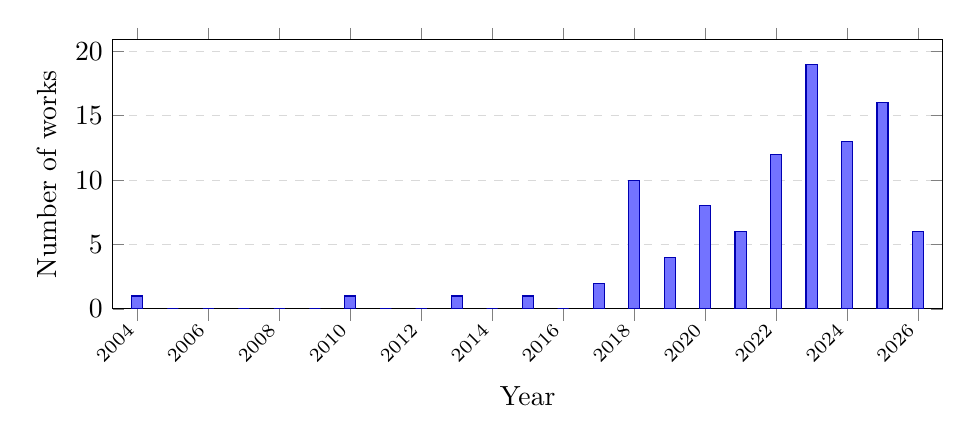
\begin{tikzpicture}
\begin{axis}[
  ybar, width=\columnwidth, height=5cm, bar width=4pt,
  xmin=2003.3, xmax=2026.7, ymin=0,
  xlabel={Year}, ylabel={Number of works},
  xtick distance=2, x tick label style={/pgf/number format/1000 sep=, rotate=45, anchor=east, font=\scriptsize},
  ymajorgrids, grid style={dashed,gray!30}, enlarge x limits=false]
\addplot[fill=blue!55, draw=blue!70!black] coordinates {(2004,1) (2005,0) (2006,0) (2007,0) (2008,0) (2009,0) (2010,1) (2011,0) (2012,0) (2013,1) (2014,0) (2015,1) (2016,0) (2017,2) (2018,10) (2019,4) (2020,8) (2021,6) (2022,12) (2023,19) (2024,13) (2025,16) (2026,6)};
\end{axis}
\end{tikzpicture}
\caption{Distribution of the surveyed works by publication year.}
\label{fig:years}
\end{figure}
\subsection{Cross-Cutting Trends and Publication Dynamics}
The corpus surveyed here spans more than two decades, from early wearable-computing demonstrations of physiological emotion recognition \cite{lisetti2004noninvasive} to speculative 2026 work on portable multimodal recognition pipelines \cite{darabkh2026exploring,site2026emotion,c2026survey,shahid2026comparative,noori2025sensitivity}. As shown in Fig.~\ref{fig:years}, publication activity is heavily skewed toward the present decade, peaking in 2023 and with roughly 35\% of the 100 reviewed works appearing in the last three years. This acceleration coincides with the maturation of low-power wearable platforms, the proliferation of consumer-grade biosensing rings and smartwatches \cite{wang2025computing,lindstrom2025wearable,li2024comparison,shahid2026comparative}, and the broader uptake of deep learning in affective computing \cite{dar2020cnn,zou2024emotion,wu2023transformer,li2025transformer}. A clear trajectory emerges across the themes: early studies established feasibility using single modalities and classical classifiers \cite{lisetti2004noninvasive,vijaya2013galvanic,setyohadi2018galvanic}; mid-period work shifted toward multimodal fusion and richer feature engineering \cite{wei2018emotion,ayata2020emotion,pinto2020multimodal,dessai2024multimodal}; and the most recent works emphasize deep representation learning, self-supervision, and transformer architectures applied to wearable or ring-form-factor sensors \cite{dissanayake2022sigrep,wu2023transformer,li2025transformer,sumanth2025bilstm}. This temporal arc mirrors broader trends in physiological computing, where the field moves from signal-specific heuristics toward end-to-end learned representations, yet the underlying sensing modalities (GSR/EDA, ECG, PPG) remain largely unchanged.

\subsection{Dominant Sensing Modalities and Techniques}
Across the five themes, galvanic skin response/electrodermal activity (GSR/EDA) and ECG emerge as the dominant and most frequently combined physiological signals for emotion inference \cite{ayata2017emotion,fan2023human,machot2019deep,bulagang2020review,damelio2025emotion,sumanth2025bilstm,dessai2024multimodal}, often supplemented with EEG \cite{houssein2022human,kwon2018electroencephalography,dar2020cnn,cimtay2020cross}, respiration, skin temperature, or PPG \cite{liu2018human,wei2018emotion,ayata2020emotion,bamonte2024determining,darabkh2026exploring}. Machine learning techniques progress from classical SVM, kNN, and Naive Bayes classifiers \cite{setyohadi2018galvanic,marinmorales2018affective,shahid2026comparative} to convolutional and recurrent architectures \cite{granados2018deep,dar2020cnn,nandini2025ensemble,liao2025emotion}, and increasingly to attention-based and self-supervised models that aim to improve cross-subject generalization \cite{zou2024emotion,dissanayake2022sigrep,wu2023transformer,li2025transformer}. A persistent methodological divide separates subject-dependent from subject-independent evaluation; several works explicitly address the generalization gap through transfer learning \cite{jacobsen2021classification}, personalized versus generalized model comparisons \cite{li2024comparison}, or subject-independent CNN design \cite{machot2019deep}, reflecting a cross-cutting recognition that physiological signals are highly idiosyncratic and that benchmark accuracy under leave-one-subject-out protocols is substantially harder to achieve than under mixed-subject splits. Fusion strategies---whether feature-level, decision-level, or hybrid---recur throughout the ML and GSR/ECG themes \cite{wei2018emotion,cimtay2020cross,dessai2024multimodal,subasi2025multimodal,zou2024emotion}, suggesting a broad consensus that no single physiological channel is sufficient and that multimodal fusion is the de facto standard, even though the specific combination of signals and fusion method varies widely across studies without clear convergence on an optimal architecture.

\subsection{Datasets, Benchmarks, and Evaluation Practices}
A small set of public datasets recurs across the ML and wearable deep learning themes, most notably AMIGOS \cite{granados2018deep} and DEAP \cite{kumar2024machine}, alongside newer multimodal corpora such as MPED \cite{song2019mped}, PhyMER \cite{pant2023phymer}, WEMAC \cite{a2022wemac}, and the stress-focused dataset of \cite{hosseini2022multimodal}. However, the overall landscape remains fragmented: many studies rely on custom, unpublished elicitation protocols (e.g., tactile multimedia \cite{raheel2020physiological}, Quranic recitation \cite{darabkh2026exploring}, naturalistic conversation \cite{zitouni2022lstm}, or virtual reality \cite{marinmorales2018affective,polo2025advancing,anon2025performance}), which complicates direct comparison of reported accuracies. Evaluation practices are similarly heterogeneous: some works report simple classification accuracy for discrete emotion categories \cite{fan2023human,setyohadi2018galvanic}, others adopt the arousal--valence dimensional model \cite{veeranki2024comparison,ayata2020emotion,moontaha2023online}, and a few explicitly compare which emotional model (categorical versus dimensional, arousal versus valence) is best supported by the underlying signal, finding that arousal-based models tend to outperform valence-based ones for EDA \cite{damelio2023exploring,damelio2025emotion}. Review and meta-analytic works \cite{khare2023emotion,shu2018review,egger2019emotion,saganowski2022emotion,c2026survey} consistently flag small sample sizes, inconsistent preprocessing, and lack of standardized benchmarks as persistent weaknesses, echoing concerns raised in systematic reviews of EDA-specific systems \cite{damelio2025emotion} and broader surveys of GSR/ECG approaches \cite{bulagang2020review}.

\subsection{Reproducibility and Methodological Gaps}
Reproducibility remains a cross-cutting weakness. Few studies in the reviewed corpus disclose code, raw signal data, or detailed hyperparameter settings, and comparative benchmarking across studies is hindered by differing electrode placements \cite{sanchezcomas2021correlation,noori2025sensitivity}, window durations \cite{bamonte2024determining}, and feature-extraction pipelines \cite{diaz2024fractal,veeranki2024comparison}. Attempts to formalize metadata and context---such as ontological modeling of EDA signal provenance \cite{zawadzka2023ontological} or incorporation of personality as context \cite{pant2023phymer}---represent nascent but still rare efforts toward standardization. The sensor hardware itself introduces another reproducibility axis: studies employing research-grade multi-channel rigs \cite{liu2018human,wei2018emotion} are difficult to compare with those using low-cost Arduino-based or consumer wearable sensors \cite{shahid2026comparative,patil2023face,baldassarri2023wearables}, and self-adjustable analog front-ends proposed to personalize GSR acquisition \cite{miranda2023self} highlight that even signal acquisition circuitry is not yet standardized. This heterogeneity is compounded by the diversity of emotion-elicitation paradigms (multimedia, VR, conversation, physical activity), each of which likely induces different autonomic response profiles, making cross-study generalization claims tentative at best.

\subsection{Positioning of Ring-Form-Factor Bioimpedance Sensing}
Relative to the broader wearable and EDA/ECG literature, bioimpedance sensing remains comparatively underexplored for emotion recognition specifically, despite its established utility for other physiological measurements such as blood pressure \cite{sel2023continuous,lindstrom2025wearable}, blood glucose \cite{sanai2021evaluation}, fluid volume \cite{noori2025sensitivity}, and physical activity \cite{jacobs2026advancing}. The ring form factor, reviewed broadly in \cite{wang2025computing} and instantiated for hemodynamic sensing in \cite{lindstrom2025wearable} and cuffless blood pressure in \cite{sel2023continuous}, offers a socially acceptable, continuous-wear alternative to chest straps or wrist bands, yet none of the reviewed works directly demonstrate bioimpedance-ring-based emotion classification; instead, the emotion-recognition literature predominantly relies on GSR/EDA and ECG/PPG sensing modalities validated in finger, wrist, or chest placements \cite{sanchezcomas2021correlation,zangroniz2017electrodermal,bamonte2024determining}. This gap suggests an opportunity at the intersection of the bioimpedance sensing theme and the wearable deep learning theme: combining the multi-parameter sensing capability of bioimpedance (capturing fluid shifts, vascular tone, and possibly sympathetic-driven impedance changes) with the self-supervised and transformer-based representation learning techniques already validated on EDA/ECG wearable data \cite{dissanayake2022sigrep,wu2023transformer,li2025transformer} could enable a new class of compact, multi-modal affective sensing devices, provided that future work addresses the reproducibility and benchmarking shortcomings identified throughout this survey.

\section{Open Challenges and Future Directions}\label{sec:challenges}
\subsection{Form-Factor Constraints and Motion Artifacts in Ring-Based Sensing}
Unlike wrist- or chest-worn platforms, a ring must accommodate electrodes, analog front-end, and power source within a few cubic centimeters while maintaining stable skin contact on a finger that is in constant, unconstrained motion. Reviews of bioimpedance measurement note that despite promising applications in activity and health monitoring, the technology continues to suffer from low spatial resolution, motion artifacts, and strong sensitivity to electrode placement and contact pressure \cite{jacobs2026advancing}. Related work on leg bioimpedance in pediatric patients shows that even small variations in electrode positioning materially change the sensitivity of the measurement to the underlying physiological change being tracked \cite{noori2025sensitivity}, which is directly relevant to a ring that cannot guarantee a fixed electrode-skin geometry across wearers or over the course of a day. Comparable concerns have driven the broader wearable vital-sign literature to favor bulkier or more constrained form factors (cuffs, chest bands, fiber-optic sensors) specifically because they offer more stable coupling \cite{sel2023continuous,lindstrom2025wearable,mayoral2021fiber,dias2018wearable}. Future ring designs will need adaptive or self-calibrating electrode interfaces, analogous to self-adjustable galvanic skin response front-ends proposed for personalized skin-conductance sensing \cite{miranda2023self}, together with on-board motion sensing to detect and compensate for artifacts in real time, and textile- or flexible-material innovations drawn from the broader wearable biosensor literature \cite{li2023advanced}.

\subsection{Weak Theoretical Grounding of Emotion Constructs in Bioimpedance Signals}
A recurring critique of electrodermal- and physiology-based emotion recognition systems is that the theoretical emotion models underlying them have received comparatively little scrutiny, with systems built opportunistically around whatever labels a dataset provides rather than a validated psychological framework \cite{damelio2025emotion,damelio2023exploring}. This is especially acute for bioimpedance ring sensing, where the physiological pathway linking impedance changes at the finger to discrete or dimensional emotion states (valence, arousal, or categorical affect) is largely unestablished and simply inherited from the electrodermal activity literature. Yet even within that literature, findings increasingly complicate the conventional assumption that skin-conductance-related signals index arousal alone: fractal analysis of electrodermal activity shows robust correlations with both arousal and valence dimensions, challenging the traditional arousal-only interpretation \cite{diaz2024fractal}. Future work should explicitly test which emotion models (categorical, circumplex, appraisal-based) are empirically supported by bioimpedance-derived features before building classifiers around them, rather than assuming direct transfer from skin conductance paradigms.

\subsection{Scarcity of Bioimpedance-Specific Emotion Datasets and Ground-Truth Labels}
Most wearable emotion recognition research draws on datasets built around EEG, ECG, or electrodermal activity; to date, no large-scale, validated bioimpedance-ring emotion dataset exists. This gap compounds a challenge already noted across the wider affective computing field: the limited availability of reliable data labels is an inherent obstacle to developing robust models for emotion recognition from wearables \cite{dissanayake2022sigrep}, and discrepancies between readily available labels and true affective states necessitate more frequent, delayed-label collection in naturalistic settings \cite{moontaha2023online}. Systematic choice of physiological measures that actually cover the elicited emotional response space is also not obvious \cite{hui2018coverage}, meaning that a ring-based bioimpedance channel may need to be co-registered with established modalities during dataset construction to establish its incremental validity. Efforts such as ontology-based metadata standards for electrodermal activity datasets \cite{zawadzka2023ontological} offer a template for how bioimpedance-ring datasets could be documented and shared consistently, and self-supervised or contrastive representation learning approaches designed for lossy, label-scarce wearable signals \cite{dissanayake2022sigrep,wu2023transformer} represent promising directions for reducing reliance on large labeled corpora.

\subsection{Generalization Across Individuals and Contexts}
Physiological responses to emotional stimuli vary substantially between individuals due to intrinsic and extrinsic factors, a problem explicitly highlighted in the context of skin-conductance sensing where a lack of self-adjustable sensors limits personalization \cite{miranda2023self}. More broadly, training a model on one group of subjects and testing it on an unseen group remains a serious open problem in emotion recognition, since different individuals may exhibit markedly different emotion-related physiological patterns \cite{machot2019deep}. Comparative studies of personalized versus generalized modeling approaches on consumer wearables likewise underscore that generalized models trained across populations can underperform relative to individually tuned ones \cite{li2024comparison}. For a bioimpedance ring intended for everyday, out-of-lab use, this challenge is magnified by finger anatomy differences, hydration state, skin temperature, and activity level, all of which can confound the bioimpedance signal independently of emotional state. Promising directions include subject-adaptive or few-shot calibration schemes, transfer learning strategies as explored for electrodermal activity classification \cite{jacobsen2021classification}, and online learning pipelines that continually adapt to a wearer's baseline \cite{moontaha2023online}.

\subsection{Disentangling Emotion-Relevant Signal from Multimodal and Confounding Physiological Variation}
Emotion expression is diverse, and different modalities capture only partial, sometimes conflicting, views of the underlying affective state; classification based purely on signals such as ECG and galvanic skin response has been shown to yield unsatisfactory precision \cite{dessai2024multimodal}, and designing networks that effectively fuse heterogeneous modal signals remains an open problem given the diversity of emotion expression \cite{zou2024emotion}. Single-modality recognition is further limited because different emotional states can be physiologically indistinguishable, or because noise specific to one modality degrades classification \cite{udahemuka2024multimodal}. For a bioimpedance ring, which inherently measures a composite signal sensitive to blood volume, hydration, sweat gland activity, and movement simultaneously, isolating the emotion-relevant component from these confounds is especially difficult, echoing observations that certain emotion categories (e.g., contempt and disgust) show only minimal relationships with physiological data in general \cite{onim2025exploring}. Multimodal fusion strategies, including attention-based neural architectures \cite{zou2024emotion} and transformer-based models designed to exploit temporal and cross-modal relationships \cite{li2025transformer,wu2023transformer}, are promising, but will require the ring's bioimpedance channel to be validated as a genuinely complementary, rather than redundant, source relative to co-located photoplethysmography or temperature sensing.

\subsection{Real-Time, On-Device Processing Under Severe Resource Constraints}
Translating bioimpedance ring sensing into continuous, everyday emotion monitoring requires on-device inference under strict power, memory, and computation budgets, a challenge broadly documented for machine learning on wearable health devices \cite{sabry2022machine}. Traditional approaches that offload processing to a paired application on a personal computer are cumbersome and lack the mobility needed for real-world affective computing \cite{mai2023real}. Work on behind-the-ear EEG devices demonstrates the feasibility of embedding machine-learning inference directly on-chip for real-time emotion recognition \cite{mai2023real}, and lightweight single-modality models, such as PPG-only predictors of arousal and valence intended for smartphone deployment \cite{darabkh2026exploring}, illustrate a viable path toward minimal-footprint inference. Extending such approaches to bioimpedance rings will require careful co-design of low-power analog front ends, efficient feature extraction, and compact classifiers capable of running within the ring's thermal and energy envelope, without sacrificing the temporal resolution needed to track dynamic affective episodes.

\subsection{Validity of Ground-Truth Labels and Ecological Validity of Elicitation}
Even with improved sensing, the field faces a persistent measurement problem: self-reported or observer-based emotion labels may not reflect true internal states, since individuals can consciously or unconsciously mask their emotions, and facial expressions, often used as a proxy ground truth, can be voluntarily controlled and therefore fail to represent genuine affect \cite{houssein2022human,saffaryazdi2022facial}. Laboratory paradigms that gather physiological signals typically require participants to remain stationary with expensive, obtrusive equipment, limiting ecological validity and making it unclear how findings transfer to naturalistic, ambulatory use of a ring \cite{gohumpu2023emotion}. Complementary biomarker approaches, such as catecholamine concentration measurement alongside physiological signals, have been explored to triangulate ground truth for specific emotions like fear, though added temporal granularity of such measures has not always improved classifier performance \cite{qu2024advancing,gutierrezmartin2022fear}. Future bioimpedance ring studies will need to combine multiple, ideally continuous and unobtrusive, ground-truth strategies, potentially including peripheral biomarker sampling \cite{zamkah2020identification}, to validate that detected signal changes correspond to genuine affective states rather than compliant self-report or social masking.

\section{Conclusion}\label{sec:conclusion}
The preceding sections have charted a broad and rapidly evolving landscape at the intersection of wearable sensing, physiological signal processing, and machine learning for affective state recognition. The taxonomy developed here spans seven interconnected strands: general machine learning approaches to emotion detection spanning facial, EEG, and multi-physiological modalities \cite{sharma2023emotion,houssein2022human,khare2023emotion,liu2018human,song2019mped}; GSR- and ECG-centric recognition pipelines that increasingly rely on deep sequence models and multidomain fusion \cite{lisetti2004noninvasive,sumanth2025bilstm,site2026emotion,hui2018coverage,dessai2024multimodal}; the dedicated electrodermal activity literature, which has matured from feature-engineering studies toward systematic meta-analyses and multimodal virtual-reality paradigms \cite{damelio2025emotion,diaz2024fractal,polo2025advancing,damelio2023exploring,cimtay2020cross}; deep learning architectures tailored to the noise and variability of everyday wearable data, including contrastive and attention-based representations \cite{saganowski2022emotion,dissanayake2022sigrep,filippini2022automated,li2024comparison,zou2024emotion}; the broader wearable vital-sign monitoring ecosystem that supplies the hardware substrate for affective sensing, notably ring-form-factor devices \cite{lindstrom2025wearable,wang2025computing,sabry2022machine,dias2018wearable,mayoral2021fiber}; emerging physiological and biochemical biomarkers such as catecholamines and sweat analytes that complement classical autonomic signals \cite{gutierrezmartin2022fear,shahid2026comparative,qu2024advancing,qu2024student,zamkah2020identification}; and finally bioimpedance sensing itself, whose demonstrated utility in blood pressure, glucose, skin conductance, and fluid-volume estimation establishes it as a versatile, multiplexable modality for miniaturized, ring-based physiological monitoring \cite{sel2023continuous,sanai2021evaluation,miranda2023self,noori2025sensitivity,jacobs2026advancing}.

Across this body of work, several consistent findings emerge. First, physiological signals---whether electrodermal, cardiac, or impedance-based---reliably encode arousal-related affective information, though valence remains comparatively harder to decode, a limitation repeatedly noted in the electrodermal activity literature \cite{damelio2023exploring,damelio2025emotion}. Second, multimodal fusion, whether combining EEG, ECG, GSR, respiration, and posture signals \cite{liu2018human,song2019mped,zou2024emotion,cimtay2020cross} or biochemical and physiological channels \cite{gutierrezmartin2022fear,qu2024advancing}, consistently improves recognition accuracy and robustness over single-signal approaches. Third, the shift from laboratory-grade equipment toward unobtrusive, wearable form factors---smartwatches, patches, and especially rings---has been accompanied by advances in deep learning that address signal noise, inter-subject variability, and the generalization gap between personalized and population-level models \cite{dissanayake2022sigrep,li2024comparison,saganowski2022emotion}. Importantly, bioimpedance has independently proven effective for monitoring blood

\bibliographystyle{IEEEtran}
\bibliography{refs}
\end{document}
